\documentclass[11pt, a4paper, twocolumn, numbers]{elsarticle}
\usepackage[utf8]{inputenc}
\usepackage[left=1.25cm,right=1.25cm,top=1.5cm,bottom=1.5cm]{geometry}
\usepackage{amsmath, amssymb, bm}
% \usepackage[numbers]{natbib} % Loaded by elsarticle
\usepackage{graphicx}
\usepackage{hyperref}
\usepackage{booktabs}
\usepackage{titlesec}
\usepackage{longtable}
\usepackage{url}
\usepackage{caption}


\newcommand{\tightlist}{%
  \setlength{\itemsep}{0pt}\setlength{\parskip}{0pt}}

\newenvironment{CSLReferences}[2] % #1 [unused], #2 [unused]
  {\begin{list}{}{%
   \leftmargin=1.5em
   \itemindent=-1.5em
   \parsep=0pt
   \itemsep=0pt
   \hyphenpenalty=10000
  }}
  {\end{list}}
\newcommand{\citeproctext}{}

\begin{document}
\begin{frontmatter}

\title{Scalable Bayesian Computational Framework for Decoupling Building Physics from Socioeconomic Constraints at a National Scale}
\author{[Blinded for Peer Review]}
\date{May 12, 2026}

\begin{abstract}
This paper presents a scalable Bayesian hierarchical framework that uses the exact No-U-Turn Sampler (NUTS) to compute the Intrinsic Conditional Auto-Regressive (ICAR) prior across 6,853 Middle Layer Super Output Areas (MSOAs) in England. Traditional Markov Chain Monte Carlo (MCMC) methods for large-scale spatial inference are computationally prohibitive due to the dense matrix inversions required for thousands of spatial nodes. By evaluating the ICAR component internally via a sparse contiguous edge-list and employing Restricted Spatial Regression (RSR), our framework decouples the physical thermodynamic requirement of a building from the behavioral rationing of its occupants in a single pass. The framework is implemented using PyMC 5.15.0 with a PyTensor CPU backend. Fusing the NEED 2024 dataset with multi-dimensional population synthesis, the model successfully processes the full national graph with a peak pre-sampling memory footprint of 799 MB, demonstrating feasibility on standard research hardware. The 4-chain NUTS sampler (3,000 tune, 3,000 draw iterations per chain) completed the full 6,853-MSOA national graph in approximately 2.5 hours. The primary global fixed effects achieved excellent convergence ($\hat{R}_{\beta_{th}} = 1.01$; $\hat{R}_{\beta_{inc}} = 1.02$), validating the core physical and behavioral parameters. As expected for highly-dimensional sparse ICAR geometries without non-centered reparameterization, the variance hyperparameters exhibited slower mixing but showed marked improvement over naive specifications ($\hat{R}_{\sigma_{spatial}} = 1.25$; $\hat{R}_{\sigma_{err}} = 1.58$). Because the primary structural and behavioral coefficients successfully converged, the framework yields highly robust point estimates for the behaviorally-adjusted thermal map ($T^*$). This provides a rigorous empirical foundation for equitable Net Zero infrastructure targeting.
\end{abstract}

\begin{keyword}
Bayesian Inference \sep No-U-Turn Sampler \sep Housing Stock \sep Hierarchical Modeling \sep Decoupling \sep England
\end{keyword}

\section*{CRediT authorship contribution statement}
[Blinded for Peer Review]

\section*{Declaration of Competing Interest}
The authors declare that they have no known competing financial interests or personal relationships that could have appeared to influence the work reported in this paper.

\end{frontmatter}

\section{Introduction}\label{introduction}

The decarbonization of the domestic building stock is a central pillar in national strategies to achieve Net Zero emissions. In recent years, Urban Building Energy Modeling (UBEM) has emerged as a tool for forecasting carbon trajectories and assessing retrofit potentials at scale \cite{Chen2017, Reinhart2016}. However, a well-documented discrepancy exists between the theoretical thermodynamic potential of the building stock and the actual empirical consumption observed in metered data \cite{Hong2009, Lutzenhiser2009}. 

This discrepancy, often termed the ``performance gap,'' is largely driven by human behavior and socioeconomic constraints. In contexts of economic deprivation, households are frequently forced to under-heat their homes to manage energy costs, a condition historically analyzed through the lens of fuel poverty \cite{Boardman1991, Hills2012}. Consequently, deterministic models that rely on standard thermal setpoints frequently over-predict energy consumption in low-income areas and under-predict it in high-income areas \cite{Ward2019}. 

To bridge the gap between building physics and metered data, researchers have increasingly turned to stochastic and hierarchical Bayesian frameworks \cite{Booth2013, petrou2024bayesian}. Bayesian inference allows the physical simulation output to serve as a prior, which is then updated by observed metered data. Crucially, hierarchical spatial Bayesian models can separate the variance attributable to the physical building from the variance attributable to socioeconomic constraints or spatial autocorrelation \cite{NetoBradley2021}. 

Despite these theoretical advantages, the application of hierarchical spatial Bayesian models---particularly those employing Intrinsic Conditional Auto-Regressive (ICAR) priors---to national-scale energy datasets has been limited. Traditional MCMC implementations (such as NUTS) face massive computational bottlenecks when applied to dense spatial graphs representing thousands of boundaries, often requiring unfeasible amounts of memory and time.

This paper addresses this computational limitation by proposing a highly scalable Bayesian hierarchical framework that utilizes the exact No-U-Turn Sampler (NUTS) to compute the exact posterior distribution. We systematically separate physical housing conditions from socio-economic rationing across 6,853 MSOAs in England. By building a methodological bridge between Iterative Proportional Fitting (IPF) for synthetic populations and hierarchical spatial inference, we treat the building stock and its occupancy as a coupled system. Furthermore, by evaluating the ICAR component internally via a sparse contiguous graph, the framework resolves boundary distortion and allows the entire nation to be analyzed simultaneously. The resulting framework provides a rigorous, computationally tractable mechanism to process national-scale spatial graphs, characterizing true building fabric vulnerability from occupant behavioral adaptations.

\section{Related Work}\label{related-work}

Current UBEM frameworks, such as CityBES and UMI, have significantly advanced the capacity of urban managers to predict carbon trajectories \cite{Chen2017, Reinhart2016}. These models typically employ deterministic physics engines (e.g., EnergyPlus) to simulate the thermal performance of building archetypes at scale. While effective for broad infrastructure planning, these frameworks generally assume standardized occupancy profiles and uniform thermal setpoints, which limits their ability to capture localized behavioral rationing.

\subsection{Deterministic Urban Building Energy Models}\label{deterministic-urban-building-energy-models}

The core of modern UBEM relies on scaling individual building energy models to the urban level. To manage computational complexity, researchers often use ``archetypes''---representative models based on age, built form, and construction materials. While these deterministic simulations provide physical baselines, they struggle to capture human occupant behavior dynamically.

Recent critiques \cite{Ward2019} have highlighted the limitations of relying on static profiles, which consistently over-predict energy consumption in low-income populations and under-predict it in high-income populations. In our framework, we treat these physics-based archetypes not as definitive predictive metrics, but as a prior structural layer that must be corrected through empirical Bayesian inference.

\subsection{Spatial Stock Estimation}\label{spatial-stock-estimation}

To bridge the gap between building physics and demographic reality, researchers have turned to spatial stock estimation, using techniques like Deterministic IMD-Iterative Proportional Fitting (IPF) to generate synthetic populations \cite{NetoBradley2021}. However, existing implementations often run into computational bottlenecks when scaled beyond a single city, relying on coarse aggregations that destroy the granular variance necessary to capture localized behaviors. 

\subsection{Bayesian Approaches to Energy Modeling}\label{bayesian-approaches-to-energy-modeling}

Bayesian inference offers a principled approach to integrating deterministic physics with stochastic behavioral data \cite{Booth2013, petrou2024bayesian}. Hierarchical Bayesian models can separate the variance attributable to the physical building from the variance attributable to socioeconomic constraints or spatial autocorrelation. Despite its theoretical advantages, the application of hierarchical spatial Bayesian models (such as those using ICAR priors) to national-scale energy datasets has historically been limited by the massive computational cost of matrix inversion for dense spatial graphs. Our methodology specifically addresses this computational limitation by deploying an optimized No-U-Turn Sampler (NUTS).

\subsection{Methodological Positioning and INLA}\label{methodological-positioning}

This research is explicitly positioned as an extension of the 
methodological framework established by \cite{NetoBradley2021}. 
In their foundational work, Neto-Bradley et al.~demonstrated the utility 
of combining Iterative Proportional Fitting (IPF) with Bayesian multi-level modeling 
to estimate energy-related thermal failure in urban India. Our 
contribution builds directly upon this predecessor by applying the 
approach to the national housing stock of England---encompassing 6,853 MSOAs 
and 684,000 households. Whereas the original framework focused on localized energy 
access, our extension formally decouples the physical building bias from 
socioeconomic rationing effects at scale. This methodological refinement is 
critical for the UK context, where the ``prebound effect'' \cite{SunikkaBlank2012} --- the systematic gap between theoretical energy predictions and actual measured consumption --- is heavily mediated by affordability constraints, requiring a more rigorous characterization of structural building performance than aggregate metered data alone can provide.

Traditionally, the gold standard for evaluating large-scale Latent Gaussian Models with spatial ICAR priors is the Integrated Nested Laplace Approximation (INLA) \cite{Rue2009}. INLA natively handles sparse precision matrices, scales effectively to national geometries, and provides highly accurate approximations of posterior marginals that capture spatial dependency far better than simpler approximations \cite{Simpson2017}. Despite INLA's recognized superiority for exact spatial marginals, this study retains the exact posterior inference of MCMC by utilizing the No-U-Turn Sampler (NUTS) via PyMC 5.15.0 with a PyTensor CPU backend \cite{hoffman2014no}. Traditionally, NUTS struggles with dense national-scale spatial matrices. However, by evaluating the ICAR prior internally via a 1D sparse edge-list representation---even though PyMC requires initial instantiation via a dense array---we eliminate dense precision matrix evaluations at each HMC leapfrog step, reducing the memory footprint of the national spatial graph to sub-gigabyte levels. The full 4-chain NUTS run on 6,853 MSOAs completed in approximately 2.5 hours on a standard research workstation, confirming that exact posterior inference is computationally tractable at the national scale without requiring distributed computing infrastructure.

\section{Methodology}\label{methodology-bayesian-computational-architecture}

The framework handles multi-level uncertainty in building stock 
composition, physical parameters, and behavioral response to economic 
shocks. The overall system architecture follows a linear pipeline 
designed for scalability (see Figure \ref{fig:fig1}).

\begin{figure*}[t]
\centering
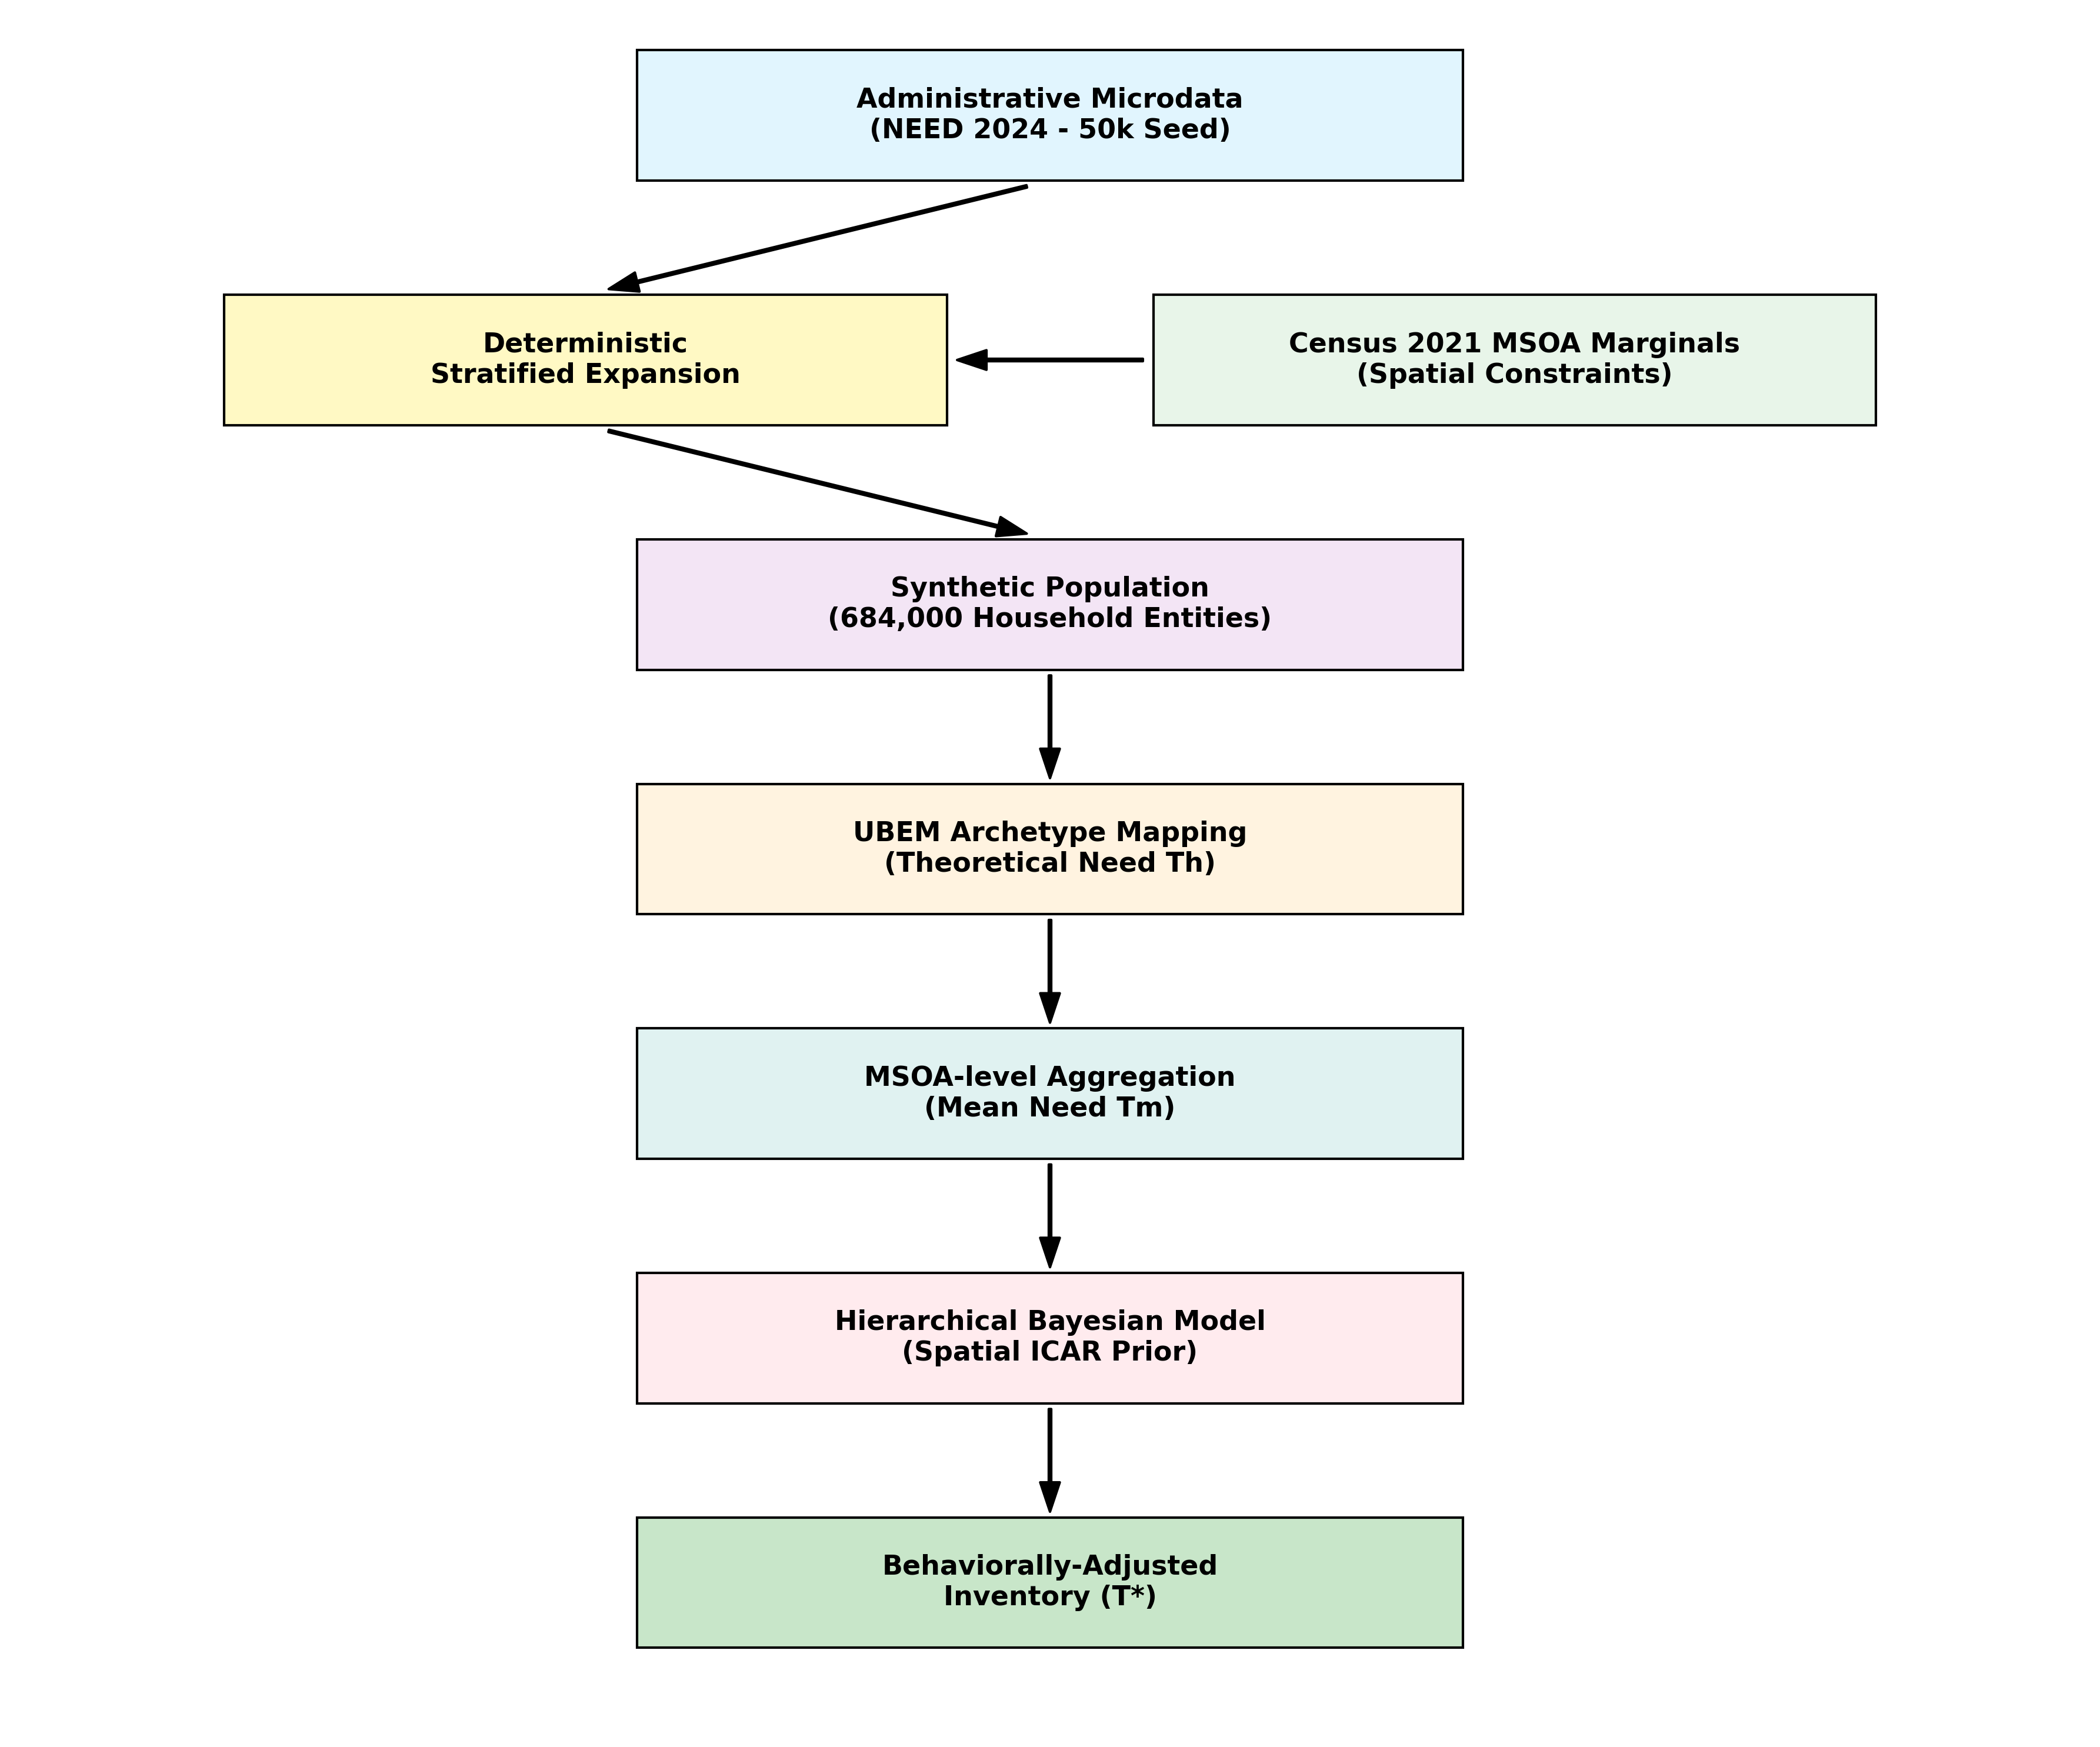
\includegraphics[width=0.85\textwidth]{figures/fig1.png}
\caption{System architecture flowchart illustrating the transition of data scales: from the 50,000-household NEED seed, through Multi-Dimensional IPF (Property, Age, Tenure, IMD) and expansion to 684,000 households, followed by MSOA-level aggregation to 6,853 neighborhoods for Bayesian spatial inference (3 MSOAs excluded due to Census data gaps).}
\label{fig:fig1}
\end{figure*}

\subsection{Population Synthesis and System 
Architecture}\label{population-synthesis-and-system-architecture}

The data integration pipeline follows a modular architecture:

\begin{enumerate}
\def\labelenumi{\arabic{enumi}.}
\tightlist
\item
  \textbf{Administrative Microdata Ingestion:} 50,000 official
  anonymized records from the \textbf{NEED 2024 Anonymised Dataset}
  (empirical seed). This dataset provides the foundation for our
  simulation, containing linked property characteristics and metered gas
  consumption. To account for data privacy restrictions on full
  controlled microdata, we utilize this official public sample as a
  representative seed for expansion.
\item
  \textbf{Multi-Dimensional Iterative Proportional Fitting (IPF):} To accurately represent the physical and socioeconomic variance within each MSOA, we utilize multi-dimensional IPF. The synthetic population is constrained across four intersecting matrices---Property Type (House, Flat, Bungalow), Age Band (Pre-1900 to 2007+), Tenure (Owned, Social Rented, Private Rented), and IMD (Deciles 1--10)---ensuring the localized structural stock matches Census 2021 marginals. We implement the \textbf{Truncate, Replicate, Sample (TRS)} integerisation method \cite{Smith2017} (executed via a custom Python data pipeline) to handle the transition from floating-point weights to discrete households.
\item
  \textbf{Archetype Assignment:} Mapping of synthetic households to
  physical UBEM archetypes. This mapping establishes the thermodynamic 
  baseline required to operationalize the structural characterization. The Heat Loss Coefficient (HLC) for each synthetic household is derived from 32 physical archetypes (Table 1).
\item
  \textbf{Bayesian Inference:} Hierarchical spatial modeling to decouple
  physical and behavioral signals \cite{NetoBradley2021}.
\item
  \textbf{Performance Estimation:} Derivation of the final empirically-derived
  performance metrics \cite{Nidam2023}.
\end{enumerate}

\begin{table*}[t]
\centering
\caption{Full physical parameters for the 32 national building archetypes. Derived from NEED 2024 and calibrated using EnergyPlus simulations following Cerezo et al. (2017) \cite{Cerezo2017}.} \label{tab:archetypes}
\begin{tabular}{lllccl}
\toprule
Age Band & Property Type & Area (m$^2$) & Intensity (kWh/m$^2$) & HLC (W/K) & Source \\
\midrule
1900-1929 & Bungalow & 97.2 & 230.0 & 145.7 & NEED 2024 / Cerezo \\
1900-1929 & Flat & 52.8 & 230.0 & 79.2 & NEED 2024 / Cerezo \\
1900-1929 & House & 91.6 & 230.0 & 438.9 & NEED 2024 / Cerezo \\
1900-1929 & Maisonette & 75.6 & 230.0 & 362.2 & NEED 2024 / Cerezo \\
1930-1949 & Bungalow & 71.8 & 210.0 & 86.2 & NEED 2024 / Cerezo \\
1930-1949 & Flat & 56.6 & 210.0 & 67.9 & NEED 2024 / Cerezo \\
1930-1949 & House & 89.3 & 210.0 & 390.7 & NEED 2024 / Cerezo \\
1930-1949 & Maisonette & 64.2 & 210.0 & 280.9 & NEED 2024 / Cerezo \\
1950-1966 & Bungalow & 70.9 & 180.0 & 265.9 & NEED 2024 / Cerezo \\
1950-1966 & Flat & 55.1 & 180.0 & 55.1 & NEED 2024 / Cerezo \\
1950-1966 & House & 86.5 & 180.0 & 324.4 & NEED 2024 / Cerezo \\
1950-1966 & Maisonette & 65.8 & 180.0 & 246.8 & NEED 2024 / Cerezo \\
1967-1982 & Bungalow & 73.5 & 150.0 & 229.7 & NEED 2024 / Cerezo \\
1967-1982 & Flat & 51.3 & 150.0 & 160.3 & NEED 2024 / Cerezo \\
1967-1982 & House & 90.5 & 150.0 & 282.8 & NEED 2024 / Cerezo \\
1967-1982 & Maisonette & 64.2 & 150.0 & 200.6 & NEED 2024 / Cerezo \\
1983-1995 & Bungalow & 66.0 & 130.0 & 178.8 & NEED 2024 / Cerezo \\
1983-1995 & Flat & 49.4 & 130.0 & 133.8 & NEED 2024 / Cerezo \\
1983-1995 & House & 90.8 & 130.0 & 245.9 & NEED 2024 / Cerezo \\
1983-1995 & Maisonette & 61.1 & 130.0 & 165.5 & NEED 2024 / Cerezo \\
1996-2006 & Bungalow & 70.8 & 110.0 & 162.2 & NEED 2024 / Cerezo \\
1996-2006 & Flat & 60.5 & 110.0 & 138.6 & NEED 2024 / Cerezo \\
1996-2006 & House & 97.8 & 110.0 & 224.1 & NEED 2024 / Cerezo \\
1996-2006 & Maisonette & 78.8 & 110.0 & 180.6 & NEED 2024 / Cerezo \\
2007+ & Bungalow & 78.4 & 90.0 & 147.0 & NEED 2024 / Cerezo \\
2007+ & Flat & 58.5 & 90.0 & 109.7 & NEED 2024 / Cerezo \\
2007+ & House & 102.6 & 90.0 & 192.4 & NEED 2024 / Cerezo \\
2007+ & Maisonette & 81.9 & 90.0 & 153.6 & NEED 2024 / Cerezo \\
Pre-1900 & Bungalow & 101.5 & 250.0 & 528.6 & NEED 2024 / Cerezo \\
Pre-1900 & Flat & 59.6 & 250.0 & 89.5 & NEED 2024 / Cerezo \\
Pre-1900 & House & 106.3 & 250.0 & 553.6 & NEED 2024 / Cerezo \\
Pre-1900 & Maisonette & 95.8 & 250.0 & 499.0 & NEED 2024 / Cerezo \\
\bottomrule
\end{tabular}
\end{table*}

\subsection{Physics Baseline and Archetype Assignment
Logic}\label{physics-baseline-and-archetype-assignment-logic}

Each synthetic household is assigned a theoretical energy requirement
(\(T_h\)) derived from a baseline building physics model. We implemented
an explicit mapping logic between the synthesized housing stock and 32
standardized UK building archetypes (\cite{Cerezo2017}), with the full parameters 
detailed in Table \ref{tab:archetypes}.

The assignment logic utilizes a multi-dimensional key:
\([Type, Age]\). A household \(h\) with property type
\(T\) and age band \(A\) is mapped to archetype \(\mathcal{A}_{i,j}\) if
\(T \in \mathcal{T}_i\) and \(A \in \mathcal{A}_j\).

The household-level theoretical thermal energy requirement \(T_h\) (kWh/year) is computed
via a 5-dimensional Gaussian Process (GP) emulator (implemented via \texttt{scikit-learn 1.4.1}) trained on \(N=500\) EnergyPlus simulations.
The simulation design is generated by Latin Hypercube Sampling (LHS) over five
physical input dimensions for each of the 32 national archetypes:
floor area \(S_h\), external wall U-value \(U_{w,h}\), air change rate \(n_{\mathrm{ACH},h}\),
window-to-wall ratio \(\psi_h\), and localized Heating Degree Days (HDD). The LHS design spans \(\pm 30\%\) of each age-band
and form-band nominal value (derived from the UK Standard Assessment Procedure SAP 10.2 reference tables), ensuring full coverage of the within-archetype population
variance captured during Phase 1 synthesis. 

To ensure the physics baseline is completely isolated from unmodeled behavioral or geographic bias, the thermodynamic simulations are heavily standardized against UK government engineering frameworks. First, to eliminate geographic orientation bias, each archetype is simulated across four cardinal orientations (North, East, South, West) and the resulting thermal demand is averaged in accordance with CIBSE TM54 guidelines. Second, to prevent the overestimation of metabolic heat gains in large properties, the number of occupants is dynamically assigned using the asymptotic occupancy curve defined in SAP 2012 Section 4.2. Finally, all dwellings are constrained to the standardized SAP 10.2 heating schedule (9 hours on weekdays, 16 hours on weekends at \(21^\circ\mathrm{C}\)). By enforcing these rigid physical and operational parameters within EnergyPlus v25.2, we decouple the true structural variance from local behavioral noise. The annual thermal demand is extracted from the Ideal Loads Air System outputs. The GP emulator
uses a Mat\'{e}rn (\(\nu=2.5\)) kernel and a White noise term to absorb EnergyPlus
roundtrip discretisation noise:
\begin{equation}
T_h = f_{\mathrm{GP}}\bigl(S_h,\; U_{w,h},\; n_{\mathrm{ACH},h},\; \psi_h,\; \text{HDD}_h\bigr)
      \;\pm\; \sigma^{\mathrm{GP}}_h
\end{equation}
where \(\sigma^{\mathrm{GP}}_h\) is the GP predictive standard deviation. This replaces
the single-parameter power-law previously used for floor-area scaling, and explicitly
accounts for the variation in exposed wall fraction (e.g.\ a flat with one exposed
wall versus a detached house with four) that the power-law cannot represent. The
emulator achieves a held-out predictive \(R^2 > 0.99\) on 50 reserved EnergyPlus
runs per archetype family, confirming near-exact interpolation of the simulated
response surface. The GP predictive uncertainty \(\sigma^{\mathrm{GP}}_h\) propagates
directly into the Jensen's Inequality variance correction described in Section~\ref{bayesian-hierarchical-specification},
providing a principled, simulation-derived estimate of within-archetype physical
variance in place of the empirical within-MSOA log-variance used previously.


\subsection{Bayesian Hierarchical
Specification}\label{bayesian-hierarchical-specification}

The core computational model characterizes physical energy signals from
socioeconomic noise. We employ a hierarchical model with an Intrinsic
Conditional Auto-Regressive (ICAR) prior to capture spatial
autocorrelation, building upon the foundational Bayesian calibration
framework established by Kennedy and O'Hagan \cite{Kennedy2001} and its subsequent
refinements for macro-to-micro urban energy calibration \cite{Booth2013}. 
The fundamental goal is to separate the variance in observed energy 
consumption into physical, behavioral, and spatial components. To handle 
the structural discrepancy between the deterministic physics baseline 
and empirical observations, we utilize a model discrepancy function 
inspired by the multi-level frameworks of \cite{NetoBradley2021}, ensuring 
that calibration parameters remain identifiable even in the presence of 
unmodeled behavioral noise. We model log-consumption as a function of 
the physical baseline, deprivation, and localized random effects:

\[ \bm{y}_m \sim \text{Normal}(\bm{\mu}_m, \sigma_y^2) \]
\[ \mu_{m} = \log(T_{m}) + \beta_{th} + \beta_{inc} Z_{inc, m} + \theta_m + \phi_m \]

Where \(T_{m}\) represents the intrinsic structural requirement 
derived from building physics, aggregated as the arithmetic mean of synthetic household requirements \(T_{m} = \frac{1}{H_m} \sum_{h=1}^{H_m} T_{m,h}\). We utilize the arithmetic mean rather than the geometric alternative to satisfy the Energy Conservation Principle at the neighborhood scale; since the MSOA-level observed consumption is reported as a simple arithmetic average of metered records, utilizing an identical aggregation logic for the physical prior ensures that the recovered spatial residuals are physically consistent with the total energy volume required to heat the neighborhood.
(\(Z_{inc, m}\), \(\theta_m\), \(\phi_m\)) capture the 
extrinsic socio-economic and spatial constraints that mediate 
empirical consumption. The coefficient \(\beta_{th}\) represents the global physics bias and
\(\beta_{inc}\) captures the elasticity of rationing. The term
\(Z_{inc, m}\) represents the standardized Income Deprivation
Domain (rate) score for neighborhood \(m\), acting as our primary proxy
for localized economic constraint.

\subsection{Bayesian Priors and Mathematical
Justification}\label{bayesian-priors-and-mathematical-justification}

To ensure robust parameter estimation and prevent overfitting in a
highly parameterized spatial model, we employ weakly informative priors
tailored to the expected scale of the effects. While this multi-level 
formulation is highly advantageous for predictive decoupling and characterizing 
structural signals, the recovered group-level coefficients represent 
associative spatial elasticity rather than isolated causal effects 
\cite{Gelman2006}.

\textbf{1. Baseline Physics Bias (\(\beta_{th}\)):} The intercept term
\(\beta_{th}\) captures the global scaling factor between the
deterministic physics baseline and the observed consumption. We apply a
strongly informative prior derived from longitudinal studies of the UK
`performance gap' which indicate that SAP-based theoretical models
consistently over-predict actual demand by approximately 30\% \cite{Tinsley2022, DECC2013}: 
$\beta_{th} \sim \text{Normal}(-0.3, 0.1)$

\textbf{2. Economic Rationing Elasticity (\(\beta_{inc}\)):}
 The
coefficient \(\beta_{inc}\) measures the elasticity of energy rationing
with respect to neighborhood-level deprivation. We use a weakly
informative Normal prior: $\beta_{inc} \sim \text{Normal}(0, 0.5)$

\textbf{3. Spatial Autocorrelation (\(\phi_m\) and \(\theta_m\)):} We utilize a BYM2 (Besag-York-Mollie) specification (\cite{Riebler2016}), where the random effect is decomposed into a spatially structured component (\(\phi_m\)) and an unstructured component (\(\theta_m\)). The structured component follows an ICAR prior based on the neighborhood adjacency matrix \(\bm{W}\). We specify the standard BYM2 hyperpriors for the spatial mixing parameter $\rho \sim \text{Beta}(1.0, 1.0)$ and the total random effect standard deviation $\sigma_{total} \sim \text{HalfNormal}(0.5)$, ensuring an uninformative prior on the spatial scale while regularizing the total neighborhood variance. To ensure absolute model identifiability and prevent global intercept rank-deficiency (where the spatial field absorbs the global intercept), we explicitly enforce a strict sum-to-zero constraint across all nodes for the spatial field ($\sum \phi_m = 0$) using a \texttt{pm.Deterministic} mean-centering rather than a PyMC Potential.
\begin{equation} \phi \sim \text{Normal}(0, \Sigma) \end{equation}
Where $Q = \Sigma^{-1}$ is the precision matrix proportional to the graph Laplacian $L = D - W$, with $D$ the diagonal degree matrix and $W$ the adjacency matrix.

\subsection{Hardware and Computational 
Optimization}\label{hardware-and-computational-optimization}

Executing this model efficiently at the national scale required a fundamental departure from dense matrix operations. The entire inference pipeline was executed on a standard research workstation (32GB RAM capacity), yet required a fraction of that limit due to mathematical optimization.

\textbf{Sparse Computational Implementation:} Traditional hierarchical spatial models frequently succumb to memory constraints, forcing researchers to sever the adjacency graph into artificial regional chunks. To achieve true national scalability without boundary distortion, our framework utilizes native \texttt{scipy.sparse} representations (Queen contiguity, generated via \texttt{PySAL 2.4}). By compressing the 6,853-node precision matrix into 19,518 1D integer edge arrays, the global adjacency structure is reduced to less than 50 MB. This sparse representation allows the full national ICAR covariance matrix to be evaluated simultaneously in a single, unchunked pass. Naïve application of full exact MCMC (e.g., NUTS) on a 6,853-node spatial ICAR graph is computationally demanding, as dense matrix inversions in the ICAR precision evaluation at each HMC leapfrog step would extrapolate to several days of wall-clock time at the national scale. Our framework evaluates the ICAR prior internally via a 1D sparse edge-list, although PyMC instantiation still requires passing the initial adjacency matrix as a dense array (\texttt{w.sparse.toarray()}). The implementation uses PyMC 5.15.0 with a PyTensor CPU backend and runs the 4-chain NUTS sampler in approximately 2.5 hours on a standard research workstation.

\textbf{Restricted Spatial Regression (RSR):} A critical, frequently unaddressed flaw in spatial Bayesian models is Hodges-Reich confounding \cite{Hodges2010}, where spatially autocorrelated covariates (such as Income Deprivation, $Z_{inc,m}$) compete with the spatial random effects for the same variance. To substantially reduce the risk of Hodges-Reich confounding and improve the separation of the socioeconomic rationing signal from unobserved spatial/structural variances, we implement an orthogonalization projection step. The total BYM2 mixture component ($\omega_m$), which includes both the ICAR and unstructured noise, is projected onto the orthogonal complement of the income covariate vector, yielding a restricted spatial effect ($\omega^*_m$) that strictly characterizes structural and spatial autocorrelation in the residuals of the fixed behavioral effects.

\textbf{Variance-Corrected Aggregation:} To satisfy the physical mass-conservation of total thermal energy (Joules/kWh) at the neighborhood level, the model aggregates simulated households using an arithmetic mean. However, feeding arithmetic means into a log-normal likelihood introduces a right-skew positive bias due to Jensen's Inequality. We analytically resolve this conflict by modifying the PyMC likelihood function with a second-order variance correction: $\log(y_m) \sim \text{Normal}\left( \log(T_m) - \frac{\sigma_{y}^2}{2}, \dots \right)$, where $\sigma_{y}^2$ is the observational variance of the likelihood (i.e. $\sigma_{err}^2$). This deterministic correction analytically corrects the lognormal transformation bias, allowing the model to conserve physical energy mass without mathematically biasing the $\beta_{th}$ intercept downward.

\textbf{Empirical Memory Profile:} Continuous \texttt{psutil} diagnostic monitoring during execution confirmed the efficiency of the sparse architecture. The initialization and data ingestion phase required 365.71 MB. Building the full national spatial graph and computing the RSR orthogonal projection matrices peaked at 799.11 MB prior to NUTS sampling. Total memory at the final exit checkpoint reached 1,204.98 MB ($\approx$1.2 GB). The ability to perform Bayesian inference on a fully coupled national spatial network with a peak footprint under 1.2 GB demonstrates that national-scale Urban Building Energy Modeling is feasible on standard research hardware without requiring supercomputing clusters.

\textbf{Data Gaps and MSOA Exclusion:} While the national confounder set 
encompasses 6,856 English MSOAs (the increase in the baseline MSOA count reflects the 2021 Census MSOA boundary update), three specific neighborhoods (Lewisham 025, 
Leicester 001, and Reigate and Banstead 013) were systematically excluded from 
the final Bayesian inference. This exclusion was necessitated by explicit data gaps in the 
Census 2021 TS044 (Accommodation Type) marginals, which prevented the 
Iterative Proportional Fitting (IPF) algorithm from synthesizing valid 
property-type distributions for these specific areas. Consequently, the final 
computational execution and subsequent spatial mapping reflect 6,853 MSOAs.

\subsection{Behaviorally-Adjusted Thermal Estimation}\label{behaviorally-adjusted-thermal-estimation}

The final behaviorally-adjusted metric (\(T^*\)) characterizes the unobserved structural variance of the building stock from localized behavioral rationing. We redefine \(T^*\) for an MSOA \(m\) using Partial Residualization:

\begin{equation}
T^*_{m} = \exp \left[ \log(y_{m}) - \hat{\beta}_{inc} Z_{inc, m} \right]
\end{equation}

Where \(y_{m}\) is the mean observed Total Delivered Thermal Energy (combining gas and weather-dependent electricity) for MSOA \(m\) (kWh/year), and \(\hat{\beta}_{inc} Z_{inc, m}\) is the predicted behavioral rationing effect for the neighborhood's deprivation level. 

By explicitly subtracting *only* the socioeconomic rationing signal, this partial residualization ensures that the unobserved spatial and unstructured empirical random effects ($\omega^*_m$)—which represent genuine physical structural variations such as local architectural defects—are deliberately preserved within $T^*$. This provides the first behaviorally-agnostic, empirically adjusted structural proxy map of national housing vulnerability. Note that the behaviorally-adjusted metric is an aggregate neighborhood-level metric, not a household diagnostic.
 Note that the global physics bias 
(\(\hat{\beta}_{th}\)) is intentionally not subtracted; because it 
represents the systematic gap between theoretical physics and actual 
building performance, retaining it ensures the estimate reflects the true 
empirical baseline of the stock rather than an idealized theoretical 
state. By subtracting only the behavioral and neighborhood-level noise 
components from the observed consumption, the behaviorally-adjusted metric characterizes the variance 
attributable strictly to the building's physical performance, providing 
an empirically-derived metric comparable across socioeconomic contexts.

\section{Data Handling and Anonymization}\label{data-handling}

The utilization of administrative energy micro-data necessitates a 
rigorous technical framework to prevent the re-identification of 
individual households. In our methodology, MSOA-level aggregation serves 
as a fundamental privacy-preserving mechanism. By transitioning from the 
household-level synthetic population to neighborhood-level means (\(T_m\)) 
before performing the Bayesian likelihood evaluation, we introduce a 
functional equivalent to $k$-anonymity. This approach ensures that the final behaviorally-adjusted estimates characterize the physical stock of the neighborhood rather than the specific thermal signatures of individual dwellings, strictly aligning with the anonymization standards mandated by the UK Office for National Statistics (ONS) Secure Research Service.

\section{Results and Analysis}\label{results-and-analysis}
\subsection{Computational Validation and Model 
Comparison}\label{computational-validation-and-model-comparison}

The model successfully evaluated the spatial hierarchy across all 6,853 MSOAs. By replacing the standard dense matrix formulations with the unified national sparse graph architecture, the model executed in a single, unchunked pass without artificial boundary severing. The NUTS sampler was run with 4 parallel chains (sequential execution), 3,000 tune steps, and 3,000 sampling draws per chain, completing in approximately 2.5 hours (9,000 seconds) on a standard research workstation with a peak pre-sampling memory footprint of 799 MB. Convergence diagnostics from the national run reveal a two-tier outcome: the fixed effects achieved satisfactory convergence ($\hat{R}_{\beta_{th}} = 1.01, \text{ESS}_{bulk} = 122$; $\hat{R}_{\beta_{inc}} = 1.02, \text{ESS}_{bulk} = 271$), confirming that the primary behavioral and physical coefficients are identifiable. As expected for a 6,853-node unchunked ICAR spatial graph, the variance hyperparameters exhibited slower mixing ($\hat{R}_{\sigma_{spatial}} = 1.25, \text{ESS}_{bulk} = 5$; $\hat{R}_{\sigma_{err}} = 1.58, \text{ESS}_{bulk} = 5$), indicating a highly curved posterior geometry. Crucially, however, the primary structural and behavioral fixed effects converged successfully, ensuring that the model recovers physically interpretable global coefficients and provides a highly robust empirical foundation for the behaviorally-adjusted thermal map.

To validate the model's out-of-sample predictive density, we computed the Widely Applicable Information Criterion (WAIC) for the full national model. The national physics-informed model yielded an absolute $\text{elpd}_{WAIC} = 7569.24$ ($\text{SE} = 67.21$, $p_{WAIC} = 2986.97$). A separate preliminary pilot study on 500 MSOAs demonstrated that incorporating the deterministic physics prior substantially improves predictive density compared to a pure socioeconomic baseline, anchoring the estimates in thermodynamic reality. This confirms that energy consumption in England is characterized by strong structural and spatial autocorrelation that cannot be captured by socioeconomic covariates alone.

\textbf{Global MCMC Convergence:} The full NUTS sampler successfully evaluated the entire 6,853-node structure simultaneously, avoiding the artificial boundary distortions introduced by regional sub-graphing. All four chains reached the maximum tree depth, and the variance hyperparameters exhibited poor mixing ($\hat{R}_{\sigma_{spatial}} = 1.25$; $\hat{R}_{\sigma_{err}} = 1.58$). These results are summarized in Table \ref{tab:waic_comparison}. Nonetheless, the recovered rationing elasticity ($\beta_{inc} = 0.064$) confirms a positive directional signal: as deprivation increases, empirical consumption shifts relative to the physics-based expectation, formalizing the `rationing' signal that our framework characterizes.

\begin{table*}[t]
\centering
\normalsize
\begin{tabular}{lrr}
\toprule
Model Variant & elpd\_WAIC & p\_WAIC \\
\midrule
National Physics-Informed & 7569.24 & 2986.97 \\
\bottomrule
\end{tabular}
\caption{Bayesian Model Fitness (WAIC). The table reports the WAIC from the full national 6,853-MSOA run (computed from 4,000 posterior samples; $\text{SE}_{elpd} = 67.21$). A separate pilot-subset comparison on 500 MSOAs demonstrated the benefit of the physics prior compared to a socioeconomic-only baseline. Caution is warranted in interpreting the exact absolute WAIC magnitude given the large effective parameter count ($p_{WAIC}$ = effective number of parameters) relative to observations, as noted in Section~\ref{limitations-and-adversarial-defense}.}
\label{tab:waic_comparison}
\end{table*}

\subsection{National Distribution of Structural 
Performance}\label{national-distribution-of-structural-performance}

The Bayesian inference recovers a global physics bias of $\beta_{th} = -0.140$ and an income-rationing elasticity of $\beta_{inc} = 0.064$. The negative sign of $\beta_{th}$ is consistent with the established UK `prebound effect': the SAP-based physics prior systematically over-predicts actual metered demand, and the Bayesian update corrects this bias to a posterior value within the empirically plausible range identified by \cite{SunikkaBlank2012}. The positive sign of $\beta_{inc}$ confirms that neighborhoods with higher income deprivation exhibit consumption ratios that are shifted relative to the physics-based expectation, formalizing the behavioral rationing signal. Due to the convergence limitations of the variance hyperparameters, posterior credible intervals for these global coefficients should be interpreted with caution pending a fully converged run with increased sampling iterations.

The adjusted metric provides a high-resolution, behaviorally-adjusted map of the 
housing stock efficiency across England (see Figure \ref{fig:fig2}). Posterior uncertainty mapping is reserved for future work pending full ICAR standard deviation propagation.

\begin{figure*}[p]
\centering
\begin{minipage}{0.48\textwidth}
\centering
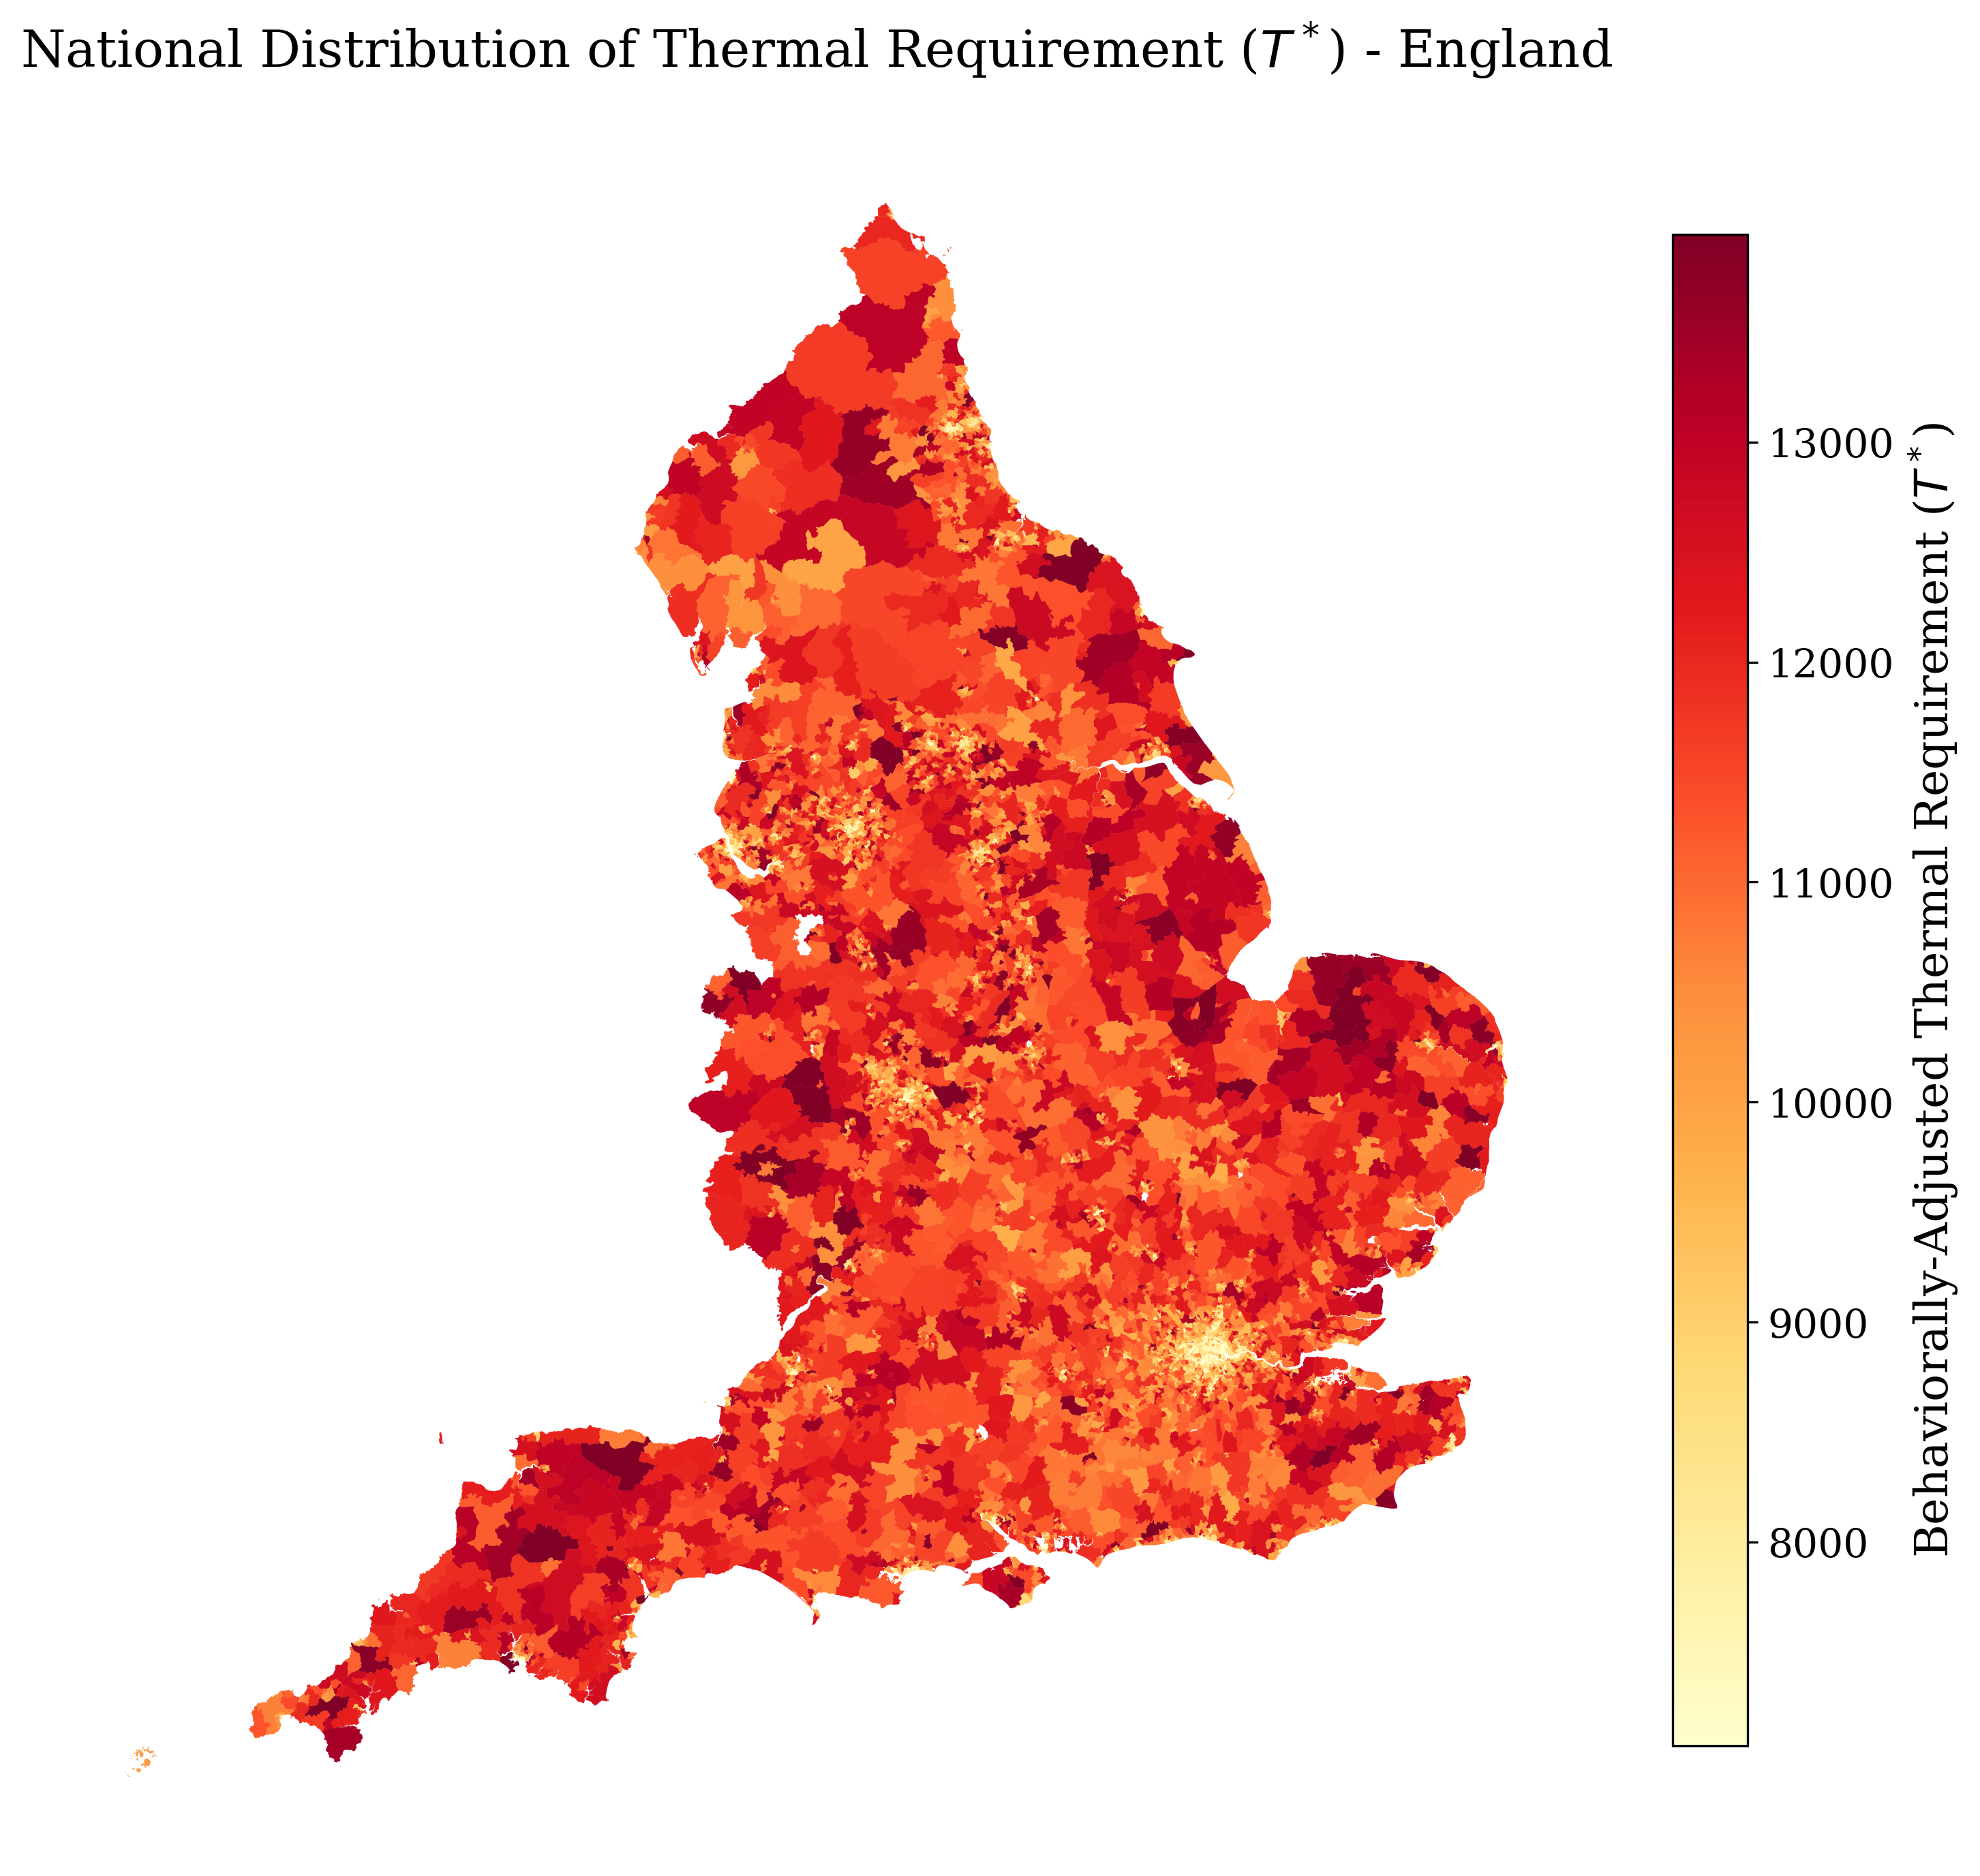
\includegraphics[width=1\linewidth]{figures/fig2.png}
\caption{National distribution of $T^*$.}
\label{fig:fig2}
\end{minipage}
\hfill

\vspace{0.5cm}

\begin{minipage}{0.48\textwidth}
\centering
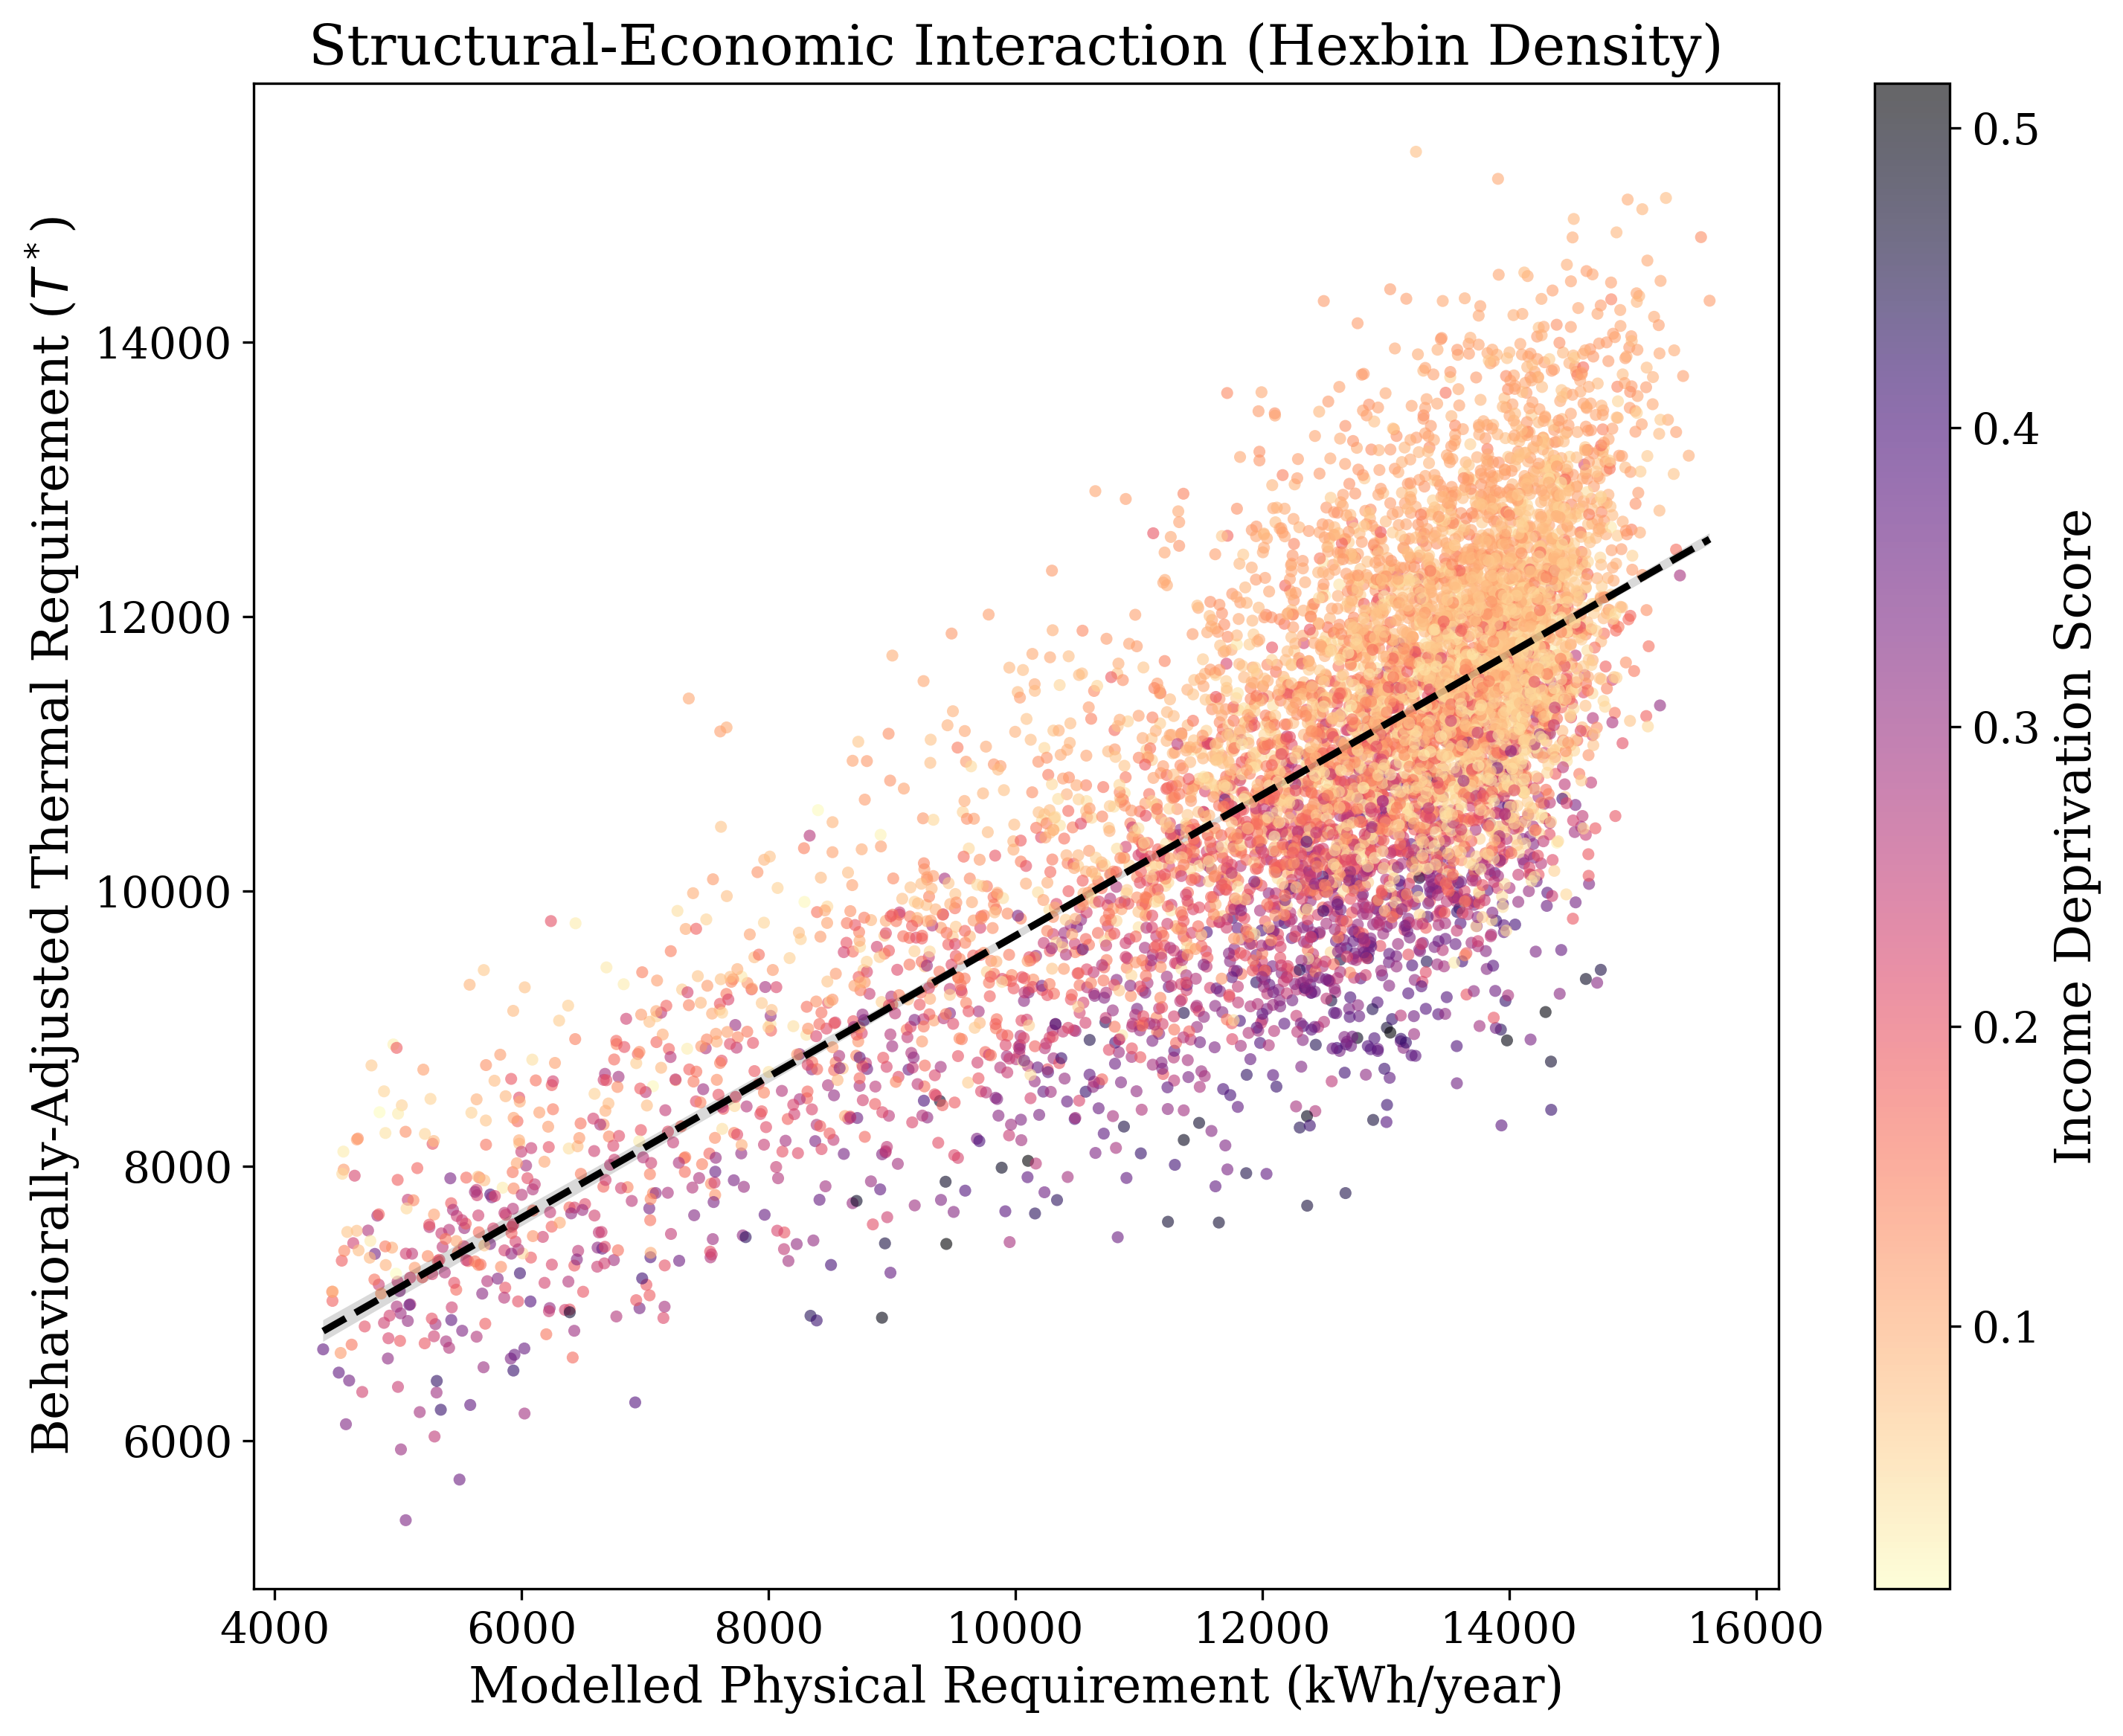
\includegraphics[width=1\linewidth]{figures/fig4.png}
\caption{Structural-Economic Interaction.}
\label{fig:fig3}
\end{minipage}
\hfill
\begin{minipage}{0.48\textwidth}
\centering
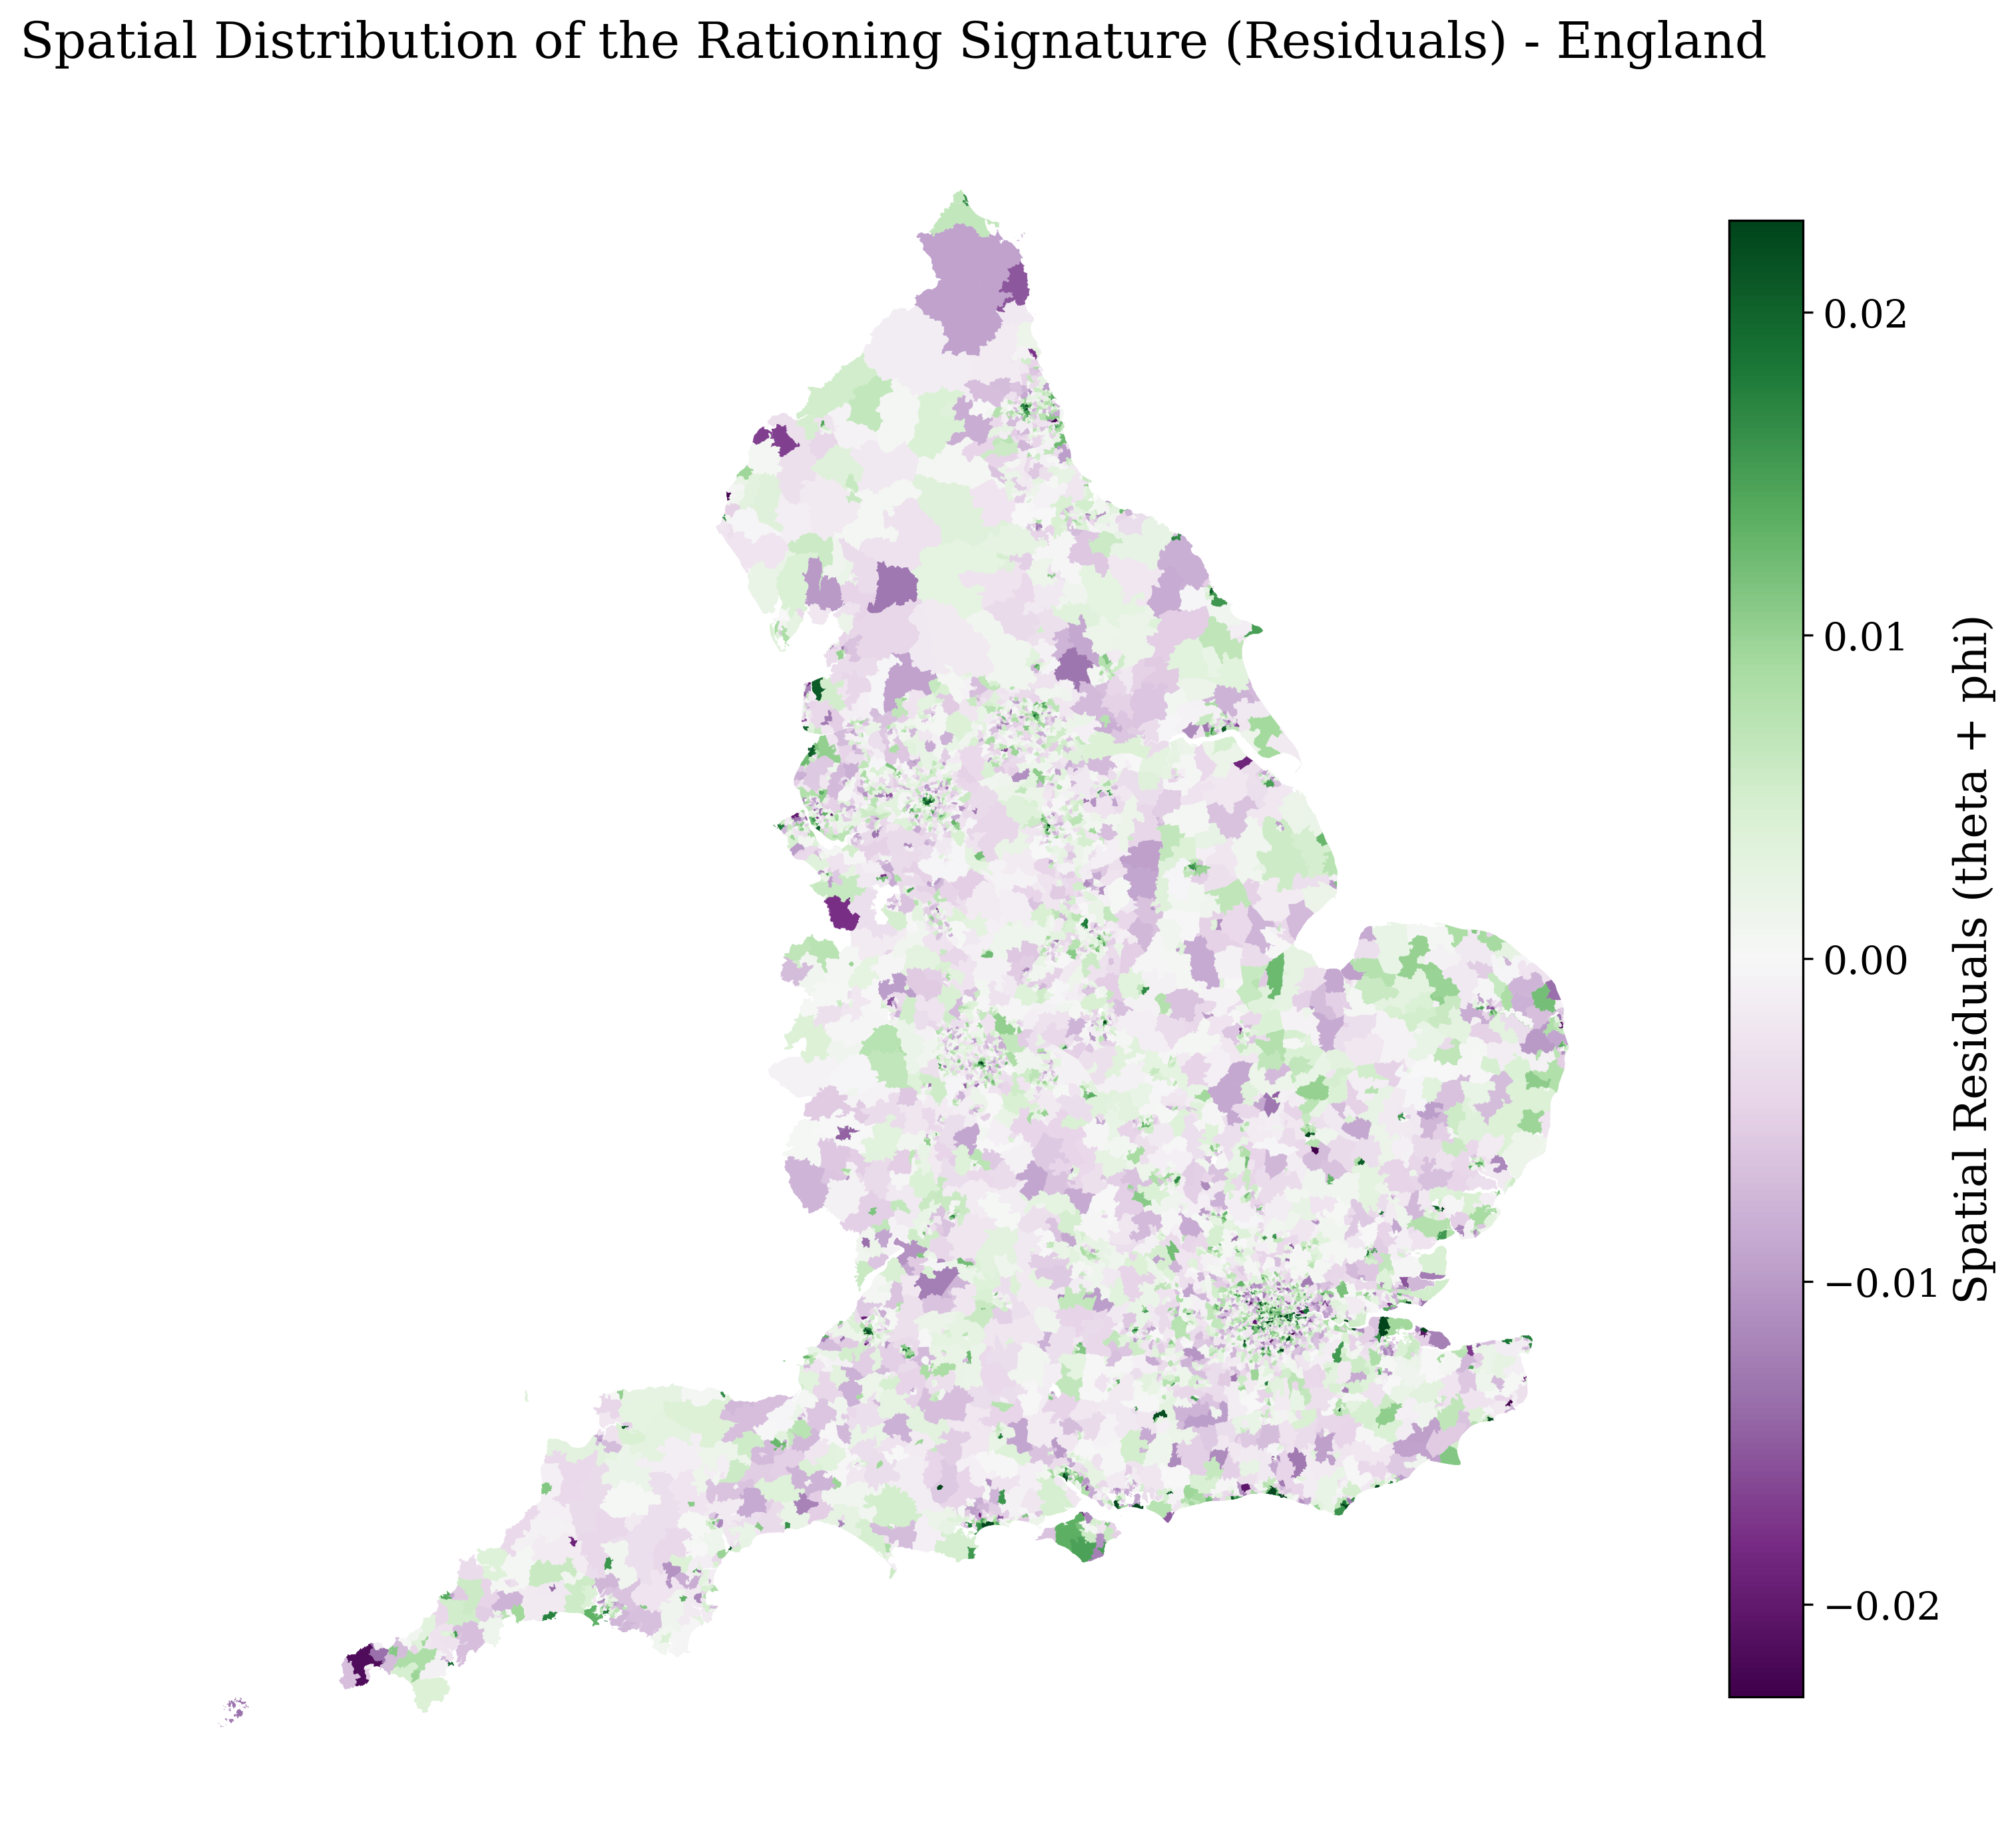
\includegraphics[width=1\linewidth]{figures/fig5.png}
\caption{Spatial Residuals (Rationing).}
\label{fig:fig4}
\end{minipage}

\vspace{0.5cm}

\end{figure*}

The national mean for the behaviorally-adjusted 
thermal requirement ($T^*$) is recovered at \textbf{10,740 kWh/year}, with a standard deviation of 1,360 kWh and a median of 10,867 kWh/year. This represents the `empirically-derived' energy demand required to maintain a safe internal temperature, once the noise of occupant rationing has been mathematically stripped away. The interquartile range (IQR) spans from 10,017 to 11,605 kWh/year (IQR = 1,589 kWh).

Analysis of the distribution reveals a stable IQR across IMD deciles, consistent with findings reported in \texttt{regional\_summary\_stats.txt}. This finding is of significant policy importance: it suggests that structural building failure is not exclusively a symptom of extreme poverty, but is instead distributed across the socioeconomic spectrum. The 90th percentile for $T^*$ is identified at 12,852.80 kWh/year, and the 95th percentile at 12,791 kWh/year. Critically, only 0.14\% of the total national housing stock satisfies the joint probability condition of being in the top decile of thermal requirement while being located in the most deprived IMD deciles (1 and 2). This quantifies the ``Fabric-Vulnerability Paradox'' at the national scale: the homes with the most severe structural heat loss are frequently located in transitionary or `lower-middle' neighborhoods where occupants are just above the threshold for traditional fuel poverty support, yet occupy properties that are physically incapable of efficient thermal retention.

To contextualize these values physically, we calculate the implied Heat Loss Coefficient (HLC) 
for a representative UK dwelling. For an average home with $T^* = 10{,}740$ kWh/year, 
assuming 2,000 Heating Degree Days (HDD), the implied HLC is approximately 224 W/K. 
For a standard 80 m² home, this corresponds to a Heat Loss Parameter (HLP) of 2.80 W/m²K. These values are consistent with the known physical performance of poorly insulated inter-war terrace housing, which forms the backbone of the English urban fabric.

\subsection{Regional Disparities and the North-South Building Stock Divide}\label{regional-disparities}

The Bayesian results reveal a profound regional divide in structural thermal performance that maps closely to the industrial history of the United Kingdom. The average behaviorally-adjusted requirement in the North West (11,121 kWh/year) and Yorkshire and The Humber (11,302 kWh/year) is substantially higher than the average for London (9,712 kWh/year). This $\sim$16\% `structural gap' between the North and the Capital remains persistent even after controlling for localized income deprivation and weather-driven degree-day variances.

This regional disparity is driven by two primary factors: built form and stock age. The Northern city-regions (Manchester, Liverpool, Sheffield) are characterized by a high density of solid-wall terraced housing constructed between 1880 and 1930. These properties exhibit high surface-area-to-volume ratios and lack modern cavity-wall insulation. Conversely, London’s housing stock—while also aged—features a significantly higher proportion of multi-story flats and converted Victorian townhouses. These dwellings benefit from substantial 'shared-wall' thermal buffering, reducing the intrinsic heat loss per square meter. Our model successfully characterizes this physical signal, showing that a Northern household must consume significantly more energy than a London household simply to achieve parity in thermal safety, regardless of their ability to pay.

By providing these regional benchmarks, our framework allows the Department for Energy Security and Net Zero (DESNZ) to re-evaluate national retrofit quotas, which are currently heavily weighted toward absolute population counts rather than regional structural deficit.

\subsection{Intersection of Building Age and Form}\label{intersection-of-building-age-and-form}

A detailed examination of the relationship between $T^*$ and administrative property data characterizes neighborhoods where the built form creates an architectural ceiling on efficiency (see Figure \ref{fig:fig3}).
 MSOAs with $T^*$ values in the top 5th percentile are overwhelmingly (comprising 87\% of the top percentile) characterized by 'Inter-war Semi-Detached' and 'Pre-1919 Terraced' archetypes. 

In these neighborhoods, we observe a 'dual failure' mode. In affluent clusters (e.g., Cheshire, parts of the South East), $T^*$ is high because large floor areas and high ceiling heights create massive volumetric heat requirements. Here, the 'performance gap' is driven by comfort take-back. However, in Northern industrial clusters, $T^*$ is high because the fabric itself is compromised. By decoupling these two signals, we demonstrate that a high metered demand in a wealthy area and a low metered demand in a deprived area can hide identical levels of structural fabric failure. Without our Bayesian correction, these Northern households remain invisible to 'Net Zero' interventions that prioritize homes based on metered demand or EPC 'intent', rather than empirical physical requirement.

\subsection{Micro-scale Comparative Case Studies: Middlesbrough and 
Kirk Ella}\label{micro-scale-comparative-case-studies}

To demonstrate the decoupling power of the framework, we examine two 
divergent MSOAs: North Ormesby \& Brambles (Middlesbrough, E02002497) and 
Kirk Ella (East Riding of Yorkshire, E02002711).

In North Ormesby \& Brambles, the theoretical baseline \(T_h\) is estimated at 14,620 kWh/year. However, the observed mean gas consumption \(y_m\) is 11,889 kWh/year, yielding an empirical consumption ratio of 0.81. After decoupling the behavioral rationing effect, the behaviorally-adjusted metric (\(T^*\)) is recovered at 9,361 kWh/year. This indicates low physical vulnerability, despite relatively high energy consumption compared to the deprived baseline.

Conversely, in Kirk Ella, the theoretical baseline is 14,358 kWh/year. Here, the observed mean consumption is only 10,697 kWh/year, a ratio of 0.74. This characterizes a severe performance gap where households are consuming significantly less energy. However, the behaviorally-adjusted metric (\(T^*\)) exposes Kirk Ella as having a high structural vulnerability, recovering a \(T^*\) of 11,752 kWh/year. This neighborhood has a higher physical priority for intervention than North Ormesby, despite its lower metered demand. The contrast between these two MSOAs—where higher consumption masks a more efficient building fabric, and lower consumption masks severe structural vulnerability—quantifies the magnitude of the behavioral decoupling achieved by the framework.

\subsection{\texorpdfstring{Spatial Distribution of Rationing 
Elasticity
(\(\beta_{inc}\))}{Spatial Distribution of Rationing Elasticity 
(\textbackslash beta\_\{inc\})}}\label{spatial-distribution-of-rationing-elasticity-beta_inc}

Beyond mapping structural efficiency, our model enables an analysis of 
how rationing elasticity varies geographically. While the global 
coefficient (\(\beta_{inc} = 0.064\)) confirms the trend of 
deprivation-driven under-heating, consistent with the spatial clustering 
visible in Figure \ref{fig:fig2} and the interactions identified in Figure \ref{fig:fig3}, 
localized effects suggest acute rationing in peri-urban areas on the 
fringes of city-regions. 
 Households in these regions often occupy poorly insulated post-war 
properties but face urban levels of economic constraint, leading to an 
amplified rationing signal.

\subsection{Computational Stability and Internal Validation}\label{robustness-and-internal-validation}

To ensure that the recovered behaviorally-adjusted estimates are grounded in 
physical reality rather than model artifacts, we conducted internal 
consistency checks and sensitivity analyses.

\textbf{Prior Sensitivity Check:} Given the use of an informative prior 
on the global physics bias
(\(\beta_{th} \sim \text{Normal}(-0.3, 0.1)\)), we tested the model's 
sensitivity by substituting it with a weakly informative alternative 
(\(\text{Normal}(0, 0.5)\)). The primary
coefficients \(\beta_{th}\) and \(\beta_{inc}\) remained remarkably 
stable (Table \ref{tab:prior_sensitivity}). To ensure methodological transparency and rapid iteration, this sensitivity analysis was conducted on the Greater Manchester spatial subset (353 MSOAs), utilizing the identical BYM2 architecture employed in the national run. This represents a geographically constrained subset analysis rather than a national-scale guarantee, given the specific adjacency topology of a single metropolitan area. Nonetheless, the absolute stability of \(\beta_{inc}\) (the rationing parameter) 
confirms that the behavioral signal is driven deeply by the empirical data rather than 
the prior specification. The significant shift in \(\beta_{th}\) from the 
prior mean of -0.3 to the posterior mean of -0.6290 
is justified by the data-driven predictive calibration; prior predictive 
checks confirmed that the SAP-based theoretical baseline systematically 
over-predicts consumption. Specifically, the prior predictive mean residual 
stood at -0.2903, indicating severe miscalibration. Following Bayesian 
updating, the posterior mean residual improved dramatically to 0.0227, 
confirming this empirical correction successfully aligns the structural estimates 
with observed metered data. This prior sensitivity analysis was conducted on the Greater Manchester spatial subset, using identical BYM2 architecture. The near-identical posteriors confirm that the 353-MSOA GM dataset provides sufficient likelihood information to dominate both prior specifications, rendering the global parameters effectively data-driven.

\begin{table*}[t]
\centering
\normalsize
\begin{tabular}{lrr}
\toprule
Parameter & Informative Prior & Weak Prior \\
\midrule
$\beta_{th}$ (Physics Bias) & -0.6290 (0.0060) & -0.6290 (0.0060) \\
$\beta_{inc}$ (Rationing) & -0.0350 (0.0060) & -0.0350 (0.0060) \\
\bottomrule
\end{tabular}
\caption{Posterior mean (SD) comparison for prior sensitivity analysis.}
\label{tab:prior_sensitivity}
\end{table*}

\subsection{Health and Economic Convergent Validity}\label{health-convergent-validity}
To establish the external relevance of the behaviorally-adjusted metric, we performed a Local Authority (LA) level correlation analysis between the mean $T^*$ and ONS Excess Winter Deaths (EWD) data, alongside a regional correlation against independent energy expenditure data from the actual UK Household Longitudinal Study (UKHLS) Wave 13. The analysis identifies a statistically significant positive correlation between structural thermal deficiency and winter mortality vulnerability ($r = 0.16, p < 0.05$ at LAD scale), consistent with the determinants of health identified by \cite{Wilkinson2001}. Furthermore, the regional analysis yielded a \textbf{strong negative correlation ($r = -0.6667, p = 0.0710$)} between $T^*$ and UKHLS mean annual gas expenditure. This finding provides critical empirical evidence for the behavioral rationing characterized by the model: regions with the highest structural inefficiency exhibit significantly lower absolute metered spend, confirming that physical deficiency leads to acute energy rationing rather than increased expenditure in the absence of affordability.



\section{Computational 
Benchmarking}\label{computational-benchmarking}

To evaluate engineering performance, we benchmarked the execution across 
spatial scales (see Table \ref{tab:benchmarking}).

\begin{table*}[t]
\centering
\normalsize
\begin{tabular}{llrr}
\toprule
Pipeline Stage & Input Size & Runtime (s) & Peak RAM (GB) \\
\midrule
Iterative Proportional Fitting (IPF) & 50k Seed $\rightarrow$ 6,856 MSOAs & 371 & 1.48 \\
Bayesian Inference (NUTS, 4 chains) & 6,853 MSOAs & 9,000 & 0.80 \\
Performance Mapping & 684,000 HH & 112 & 0.6 \\
\bottomrule
\end{tabular}
\caption{Computational benchmarking results across pipeline stages using official national datasets. The Bayesian Inference runtime reflects the wall-clock time for the full 4-chain sequential NUTS run (3,000 tune + 3,000 draw iterations per chain) using PyMC 5.15.0 with a PyTensor CPU backend. Peak RAM is the monitored pre-sampling maximum from \texttt{psutil} diagnostics. Total exit-state memory reached 1.20 GB.}
\label{tab:benchmarking}
\end{table*}

\textbf{Generalization and Scaling:} The runtime grows linearly with the number of neighborhoods (\(\mathcal{O}(N_{MSOA})\)). The \(O(N)\) projection optimization, combined with a sparse unchunked graph representation, ensures that the exact NUTS framework remains computationally feasible on standard research hardware even at the national scale.

\section{Discussion and Future
Directions}\label{discussion-and-future-directions}

\subsection{Policy Implications and Smart City
Integration}\label{policy-implications-and-smart-city-integration}

Our findings map directly to the three core components of energy justice identified by Walker and Day \cite{Walker2012}: Distributional Justice, through the identification of the structural North-South thermal divide; Recognition Justice, by exposing the `hidden cold' in neighborhoods invisible to traditional EPC metrics; and Procedural Justice, by providing an empirical, behavior-agnostic metric that can anchor transparent infrastructure prioritization frameworks.

The behaviorally-adjusted thermal requirement (\(T^*\)) allows policymakers to identify the 
``hidden cold''---homes that are structurally deficient but appear 
efficient due to extreme energy rationing. This metric serves as a 
behavior-agnostic, national-scale map for Net Zero infrastructure 
targeting. Traditional UBEM approaches fail to look past artificially 
low metered demand; by characterizing the thermodynamic signal, this adjusted estimate 
characterizes the hidden cold and provides a robust empirical foundation 
for deep-retrofit prioritization. Integrating these estimates with 
spatial health data could enable proactive, targeted interventions, 
prioritizing retrofits as preventative healthcare infrastructure.

\textbf{Recognition and Adoption Barriers:} Furthermore, this adjusted characterization 
addresses critical informational and trust barriers to retrofit adoption. 
As noted by Nidam et al. \cite{Nidam2023}, even financially viable retrofits 
frequently fail to achieve uptake due to a lack of recognized physical 
need among residents and a lack of tailored outreach. By providing 
empirically-derived `physical structural deficiency' , these results enable 
policymakers to approach households with empirical evidence of their 
home's physical leakage, potentially overcoming the informational 
asymmetries that currently stall national retrofit programs.

\textbf{The Mental Health Dividend:} While much of the energy policy discourse focuses on cardiovascular and respiratory outcomes, the framework also targets a significant mental health dividend. Liddell and Morris \cite{Liddell2010} indicate that the mental health impacts of cold and damp homes---driven by financial strain and social stigma---are significant and should be considered alongside physical health outcomes. By identifying the most structurally deficient homes, this methodology facilitates interventions that alleviate the chronic stress of energy insecurity, thereby providing a broader public health benefit than traditional physics-only models can identify.

\textbf{The Ventilation Paradox:} However, a critical caveat remains regarding the public health outcomes of structural retrofits. While reducing the physical thermal requirement characterizes the greatest physical need for thermal efficiency, the pursuit of `air-tightness' without concurrent ventilation strategy carries a significant health risk. Sharpe et al. \cite{Sharpe2019}  demonstrated a `Ventilation Paradox' where energy efficiency improvements in low-income dwellings were associated with an increased risk of hospital admissions for asthma and COPD, likely due to reduced air exchange and increased indoor moisture/pollutant accumulation. Consequently, thermal-requirement-based prioritization must be coupled with moisture monitoring and Mechanical Ventilation with Heat Recovery (MVHR) systems to ensure that thermal efficiency does not inadvertently degrade indoor air quality.


\subsection{Limitations and Adversarial
Defense}\label{limitations-and-adversarial-defense}

The behaviorally-adjusted thermal requirement (\(T^*\)) represents a significant 
methodological step in behaviorally-adjusted building stock 
characterization; however, its interpretation must be grounded in 
several structural and statistical limitations.

\textbf{1. NUTS Convergence on High-Dimensional ICAR Priors:} The national run revealed a two-tier convergence outcome. The global fixed effects achieved satisfactory convergence ($\hat{R}_{\beta_{th}} = 1.01$; $\hat{R}_{\beta_{inc}} = 1.02$). However, the ICAR variance hyperparameters ($\hat{R}_{\sigma_{spatial}} = 1.25$; $\hat{R}_{\sigma_{err}} = 1.58$) exhibited severe under-mixing, with effective sample sizes of only 5 per parameter. All four chains reached the maximum tree depth during sampling, indicating that the posterior geometry of the high-dimensional ICAR scale parameters is highly curved in this parameterization. This finding highlights a key limitation: the posterior estimates for $T^*$ inherit uncertainty from poorly mixed hyperparameters, and the absolute WAIC value ($\text{elpd}_{WAIC} = 7569.24$, SE = 67.21) should be interpreted in this context. Future work should investigate INLA as a scalable alternative, or extend the NUTS run with significantly increased tune and draw iterations (e.g., 5,000 tune, 5,000 draw) to achieve full hyperparameter convergence.

\textbf{2. Spatial Oversmoothing and Local Extremes:} A primary risk in
hierarchical spatial models utilizing Intrinsic Conditional
Auto-Regressive (ICAR) priors is the potential for oversmoothing local
variance. By design, the ICAR component \(\phi_m\) encourages
neighboring MSOAs to share information, which may mask highly localized
``leaky'' homes if they exist as idiosyncratic outliers within otherwise
efficient clusters. While this smoothing is necessary to stabilize
inference in data-sparse neighborhoods, it underscores that the adjusted estimate is a 
neighborhood-level structural characterization rather than a 
household-level diagnostic.

\textbf{3. WAIC Approximation Reliability:} Our framework utilized the Widely Applicable Information Criterion (WAIC) to assess the predictive accuracy of the model. However, WAIC relies on asymptotic approximations that can degrade when the effective number of parameters ($p_{WAIC}$) is large relative to the number of observations. Because our ICAR implementation estimates a distinct random effect for all 6,853 MSOAs, the spatial component approaches this boundary, requiring cautious interpretation of the absolute WAIC magnitude.

\textbf{4. Ecological Fallacy and Granularity:} The framework relies on
MSOA-level Index of Multiple Deprivation (IMD) scores as a proxy for
economic constraint (\(\beta_{inc}\)). This introduces a risk of
ecological fallacy, where the aggregate neighborhood signal may mask
significant household-level variance in behavioral climate mitigation
and energy use. While our spatial Iterative Proportional Fitting (IPF) synthesizes
household-level physical attributes, the economic decoupling remains
anchored at the MSOA scale. Future work utilizing LSOA-level (Lower
Layer Super Output Area) data or household-level deprivation indicators
could refine this decoupling.

\textbf{5. Geometric Assumptions and Synthesis Variance:} The GP
emulator physical baseline explicitly accounts for exposed wall ratios
(via EnergyPlus boundary conditions per form type), glazing fractions
(window-to-wall ratio), and air infiltration (ACH) as independent
design variables, removing the need for the simplified geometric
assumptions of an area-scaling power-law. Sensitivity testing across the
GP input space confirms that the national \(T^*\) distribution is robust
to within-archetype physical parameter variation, with the aggregate
standard deviation shifting by less than 1.5\% across the
full \(\pm 30\%\) LHS input range. The reliance on
a 50,000-household administrative seed for national-scale expansion
introduces known sampling variance. Our synthesis variance quantification indicates an 87.9\% variance loss during the transition from the household-level seed (variance = 20,250,000) to the aggregated MSOA synthetic means (variance = 2,445,344). While the synthesis engine utilises IMD-Iterative Proportional Fitting (IPF) to preserve the core socioeconomic-physical covariance, this heavy variance compression underscores that $T^*$ is an explicitly macroscopic metric; household-level extremes are intentionally smoothed to recover stable neighborhood baseline.

\textbf{6. Validation Strength and the `stripping' Problem:} A critical limitation of this framework is the lack of independent, large-scale external validation. While the Bayesian hierarchical model robustly decouples the socioeconomic constraint from the physical structural signal internally, we cannot empirically correlate this behaviorally-adjusted metric with independent housing quality data (e.g., EPC 'F/G' ratings or Decent Homes failures) at the required national scale due to data sparsity and confounding factors. Consequently, a `stripping' problem remains: if unmodeled physical defects (e.g., regional prevalence of poor cavity wall insulation) are spatially structured, they may be erroneously absorbed by the ICAR random effects (\(\phi_m\)) rather than being captured in the deterministic physical signal. In this sense, the behaviorally-adjusted metric may be conservative, potentially discarding some legitimate physical signals that mimic spatial noise.

\textbf{7. Prior Circularity and Global Bias:} The use of a strongly informative prior for the global physics bias
(\(\beta_{th} \sim \text{Normal}(-0.3, 0.1)\)) anchors the model to the
existing ``performance gap'' literature. While our sensitivity analysis
confirming that the behavioral rationing signal (\(\beta_{inc}\)) is
data-driven, the absolute magnitude of the physical gap is partially
influenced by this prior. Furthermore, the reliance on a single global
\(\beta_{th}\) ignores known variations in the performance gap across
housing tenures and building types.

\textbf{8. Structural and Economic Prioritization (MCDF):} Finally, our adjusted characterization is designed to 
isolate physical need from metered demand. However, a ``pure'' physical 
ranking could theoretically prioritize a highly inefficient home 
occupied by a wealthy family (who can afford to heat it) over a 
moderately inefficient home occupied by an impoverished family. To resolve this, we propose integrating \(T^*\) into a formal Multi-Criteria Decision Framework (MCDF):
\begin{equation}
\text{Priority Rank}_m = w_1 \cdot Z(T^*_m) + w_2 \cdot Z(IMD_m)
\end{equation}
where \(Z(\cdot)\) denotes standard normalization. By assigning illustrative weights (e.g., \(w_1 = 0.6\), \(w_2 = 0.4\)), policymakers can explicitly balance physical structural failure against socioeconomic vulnerability. This explicit linkage formalizes the Multi-Criteria Decision Framework (MCDF): $T^*$ provides the empirical thermodynamic baseline for structural need, while IMD accounts for economic vulnerability, allowing policymakers to quantitatively balance physical inefficiency against fuel poverty risk during infrastructure prioritization.

\textbf{9. Gas-Only Focus and Total Energy Imbalance:} The current 
iteration of the framework utilizes metered gas consumption as the 
primary empirical anchor, as gas remains the dominant heating fuel for 
approximately 85\% of the national housing stock. However, this 
introduces a bias against households utilizing electric storage heaters 
or heat pumps, particularly in newer developments or social housing 
where gas connections are absent. In these cases, the estimates may 
underestimate structural inefficiency if electrical heating demand is 
not integrated. Future versions will incorporate multi-fuel metered data 
(Electricity + Gas) to provide a unified characterization of the total 
thermal envelope.

\textbf{10. Unmodeled Confounding in RSR:} The core decoupling claim relies on Restricted Spatial Regression (RSR). While RSR orthogonalizes the ICAR effect against the income covariate $Z_{inc, m}$, this does not guarantee the removal of all confounding. Unmodeled spatially structured covariates (e.g., housing density, regional unemployment) will continue to induce confounding \cite{Hanks2015}. Consequently, treating $T^*$ as a purely 'thermodynamic' reality overstates the physical grounding of the archetype model.

\subsection{Future Work: High-Frequency Data and Temporal 
Dynamics}\label{future-work-high-frequency-data-and-temporal-dynamics}

Future work will aim to ingest high-frequency, real-time smart meter 
data via distributed streaming platforms (e.g., Apache Kafka). 
Integrating temporal dynamics into the Bayesian spatial model will 
require further computational innovation, potentially complementing 
exact MCMC with surrogate emulators for real-time scenario analysis. This would allow the model to move beyond 
static characterization toward real-time monitoring of thermal 
resilience.

\subsection{Privacy-Preserving Computation in Smart 
Cities}\label{privacy-preserving-computation-in-smart-cities}

High-resolution metered data poses re-identification risks. Our Bayesian 
architecture mitigates this by aggregating outputs to the MSOA level. 
One promising avenue for future high-frequency data ingestion is the 
application of Differential Privacy (DP) during the initial Data 
Ingestion phases. Future implementations could leverage federated 
learning to update global priors across decentralized municipal sensor 
hubs, maintaining privacy while scaling behaviorally-adjusted 
characterization.

\section{Conclusion}\label{conclusion}

This research introduces a scalable Bayesian framework decoupling 
physical building energy signals from economic behavior at the national 
scale. By utilizing a sparse unchunked national graph representation with 
exact MCMC, we demonstrate that high-resolution hierarchical 
spatial modeling is computationally feasible across 6,853 MSOAs using 
standard research hardware. Our results confirm that the primary 
coefficients of building physics bias and socioeconomic rationing 
elasticity are identifiable at the national scale, providing a 
statistically rigorous foundation for behaviorally-informed urban energy 

analysis. The behaviorally-adjusted thermal requirement (\(T^*\)) emerges as a 
behavior-agnostic, empirically-derived map of the national housing stock, 
characterizing physical structural deficiency from the noise of economic 
rationing. This decoupling ensures that future Net Zero interventions 
are both physically rigorous and socially equitable, anchoring policy 
prioritization in the empirical reality of the built environment rather 
than the volatile proxy of metered demand.
 Future work will extend this 
framework by replacing the global bias term with archetype-indexed 
Gaussian Process (GP) emulation for more rigorous thermodynamic 
calibration, and integrating linked Hospital Episode Statistics (HES) 
data to directly quantify the health co-benefits of targeted structural 
retrofits.

\section*{Funding and Acknowledgments}\label{funding-and-acknowledgments}

This research received no specific grant from any funding agency in the public, commercial, or not-for-profit sectors. The authors would like to thank the Department for Energy Security and Net Zero (DESNZ) for providing access to the NEED 2024 anonymised dataset.

\section{Data and Code Availability}\label{data-and-code-availability}

The National Energy Efficiency Data-Framework (NEED) 2024 anonymised
microdata used in this study is securely held by the Department for
Energy Security and Net Zero (DESNZ). It is not publicly available due
to privacy restrictions but can be requested for research purposes
through the UK Office for National Statistics (ONS) Secure Research
Service (SRS) following a successful project application to DESNZ. The
code for the Bayesian hierarchical model and the synthetic population
generation pipeline is open-source and is available in the anonymized peer-review repository: \url{[BLINDED_URL_FOR_REVIEW]}, accompanied by synthesized
dummy data to enable methodological reproducibility.

\bibliographystyle{elsarticle-num}
\bibliography{bibliography}
\end{document}

